\section{引言}
众所周知,chromium是多线程框架的,整个chromium浏览器包括四类进程:browser主进程、render渲染进程、GPU进程和插件进程。
本文所要讲述的chromium事件处理流程主要牵涉到其中的两种进程:browser进程和render进程。

事件处理的大体流程是由browser进程接收并传递给render进程处理。
然而我们知道render会不止一个,那么browser进程如何获取事件?
又如何传递给特定的render进程?render进程如何处理事件消息?我们下面就通过分析代码来一一探明。

chromium系统有多个平台的实现,而每个平台都有自己不同的事件管理方式,chromium也会有一些平台相关的代码。
本文目前主要是研究Linux平台相关的实现,其他平台后续再做研究。
chromium中的事件也有许多类型,如按键事件、鼠标事件、滚轮事件等等。
本文也只是以按键事件为例研究,在以下内容中,如无特殊说明,事件均指的是按键事件。

\section{按键事件获取流程}
\begin{figure}[H] 
  \centering 
  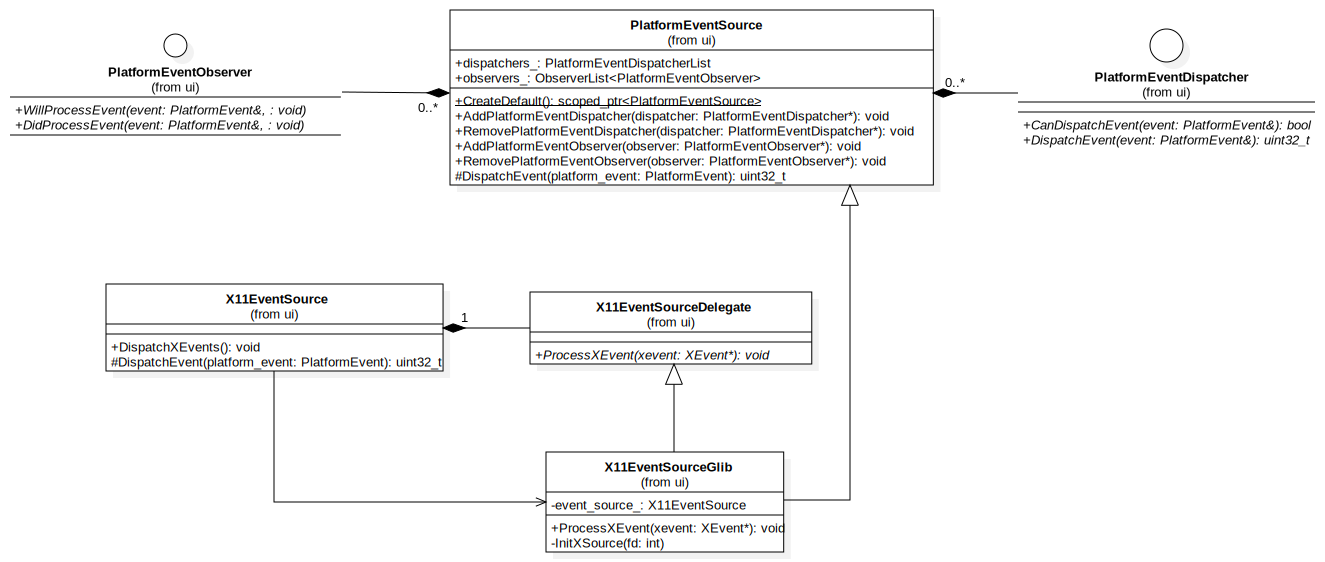
\includegraphics[width=\textwidth]{image/event_study/linux_event_source_class.pdf} 
  \caption{chromium linux平台事件源静态类图} \label{fig:linux_event_source_class} 
\end{figure}

如第图~\ref{fig:linux_event_source_class}所示:
chromium对事件源抽象了一个PlatformEventSource类表示,不同的平台继承该类实现自己平台的子类。
不过,目前发现仅有Linux平台实现了其子类X11EventSource与X11EventSourceGlib。
Windows和Android都未采用该方法。

\begin{figure}[H] 
  \centering 
  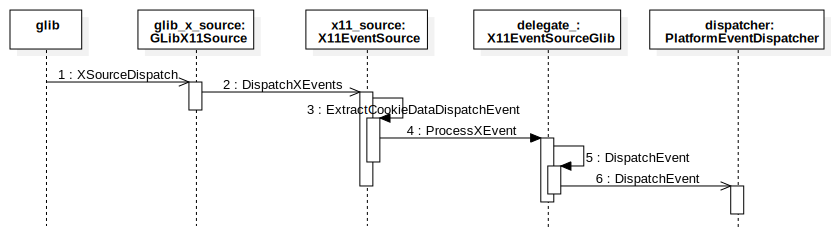
\includegraphics[width=\textwidth]{image/event_study/linux_get_event_from_source.pdf} 
  \caption{chromium linux平台事件获取时序图} \label{fig:linux_get_event_from_source} 
\end{figure}

browser进程获取按键事件的调用时序图如图~\ref{fig:linux_get_event_from_source}所示:
\begin{itemize}
  \item 在browser进程启动时,会创建一个线程循环调用g\_main\_context\_iteration方法。其作用是驱动glib检查事件,如果有事件发生,则glib会调用初始化时注册的XSourceDispatch回调来将事件传递给PlatformEventSource的子类。
  \item 第5步调用时是调用的父类PlatformEventSource方法,将事件传递给PlatformEventDispatcher。
\end{itemize}

\begin{spacing}{1.0}
\begin{lstlisting}[language={C++}]
  for (;;) {
    // Don't block if we think we have more work to do.
    bool block = !more_work_is_plausible;

    more_work_is_plausible = g_main_context_iteration(context_, block);
    if (state_->should_quit)
      break;

    more_work_is_plausible |= state_->delegate->DoWork();
    if (state_->should_quit)
      break;

    more_work_is_plausible |=
        state_->delegate->DoDelayedWork(&delayed_work_time_);
    if (state_->should_quit)
      break;

    if (more_work_is_plausible)
      continue;

    more_work_is_plausible = state_->delegate->DoIdleWork();
    if (state_->should_quit)
      break;
  }
\end{lstlisting}
\end{spacing}

\section{按键事件传递流程}
这里的按键传递流程是指browser进程从事件源处取得事件之后将其传递给特定的render进程的过程。
这里研究的是使用chromium的aura窗口系统的流程,平台是Linux平台,
然而据初步研究Windows和Android也是使用同样的流程,只是传入事件的位置不同罢了。

%---------------------------------------------------------------------

\begin{figure}[H] 
  \centering 
  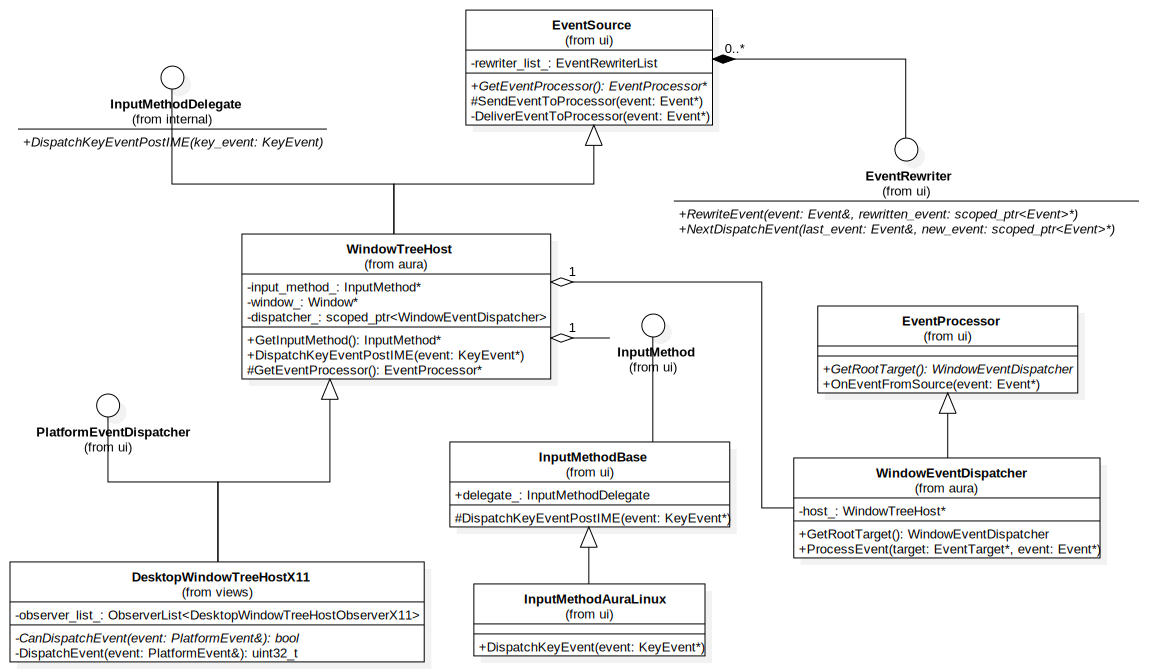
\includegraphics[width=\textwidth]{image/event_study/browser_event_dispatch_class_1.pdf} 
  \caption{chromium browser进程事件传递静态类图-1} \label{fig:linux_event_dispatch_class_1} 
\end{figure}

图~\ref{fig:linux_event_dispatch_class_1}是按键事件从PlatformEventSource到按键分发到特定window之前,
所涉及的主要类的静态类图。
\begin{itemize}
  \item DesktopWindowTreeHostX11类实现PlatformEventDispatcher接口,同时又继承了WindowTreeHost和EventSource。
  这样DesktopWindowTreeHostX11类在broeser进程中就扮演了重要的角色,可谓身兼数职。
  在事件处理流程上看它既是PlatformEventSource的dispatcher,又是UI系统的EventSource。
  \item EventSource中包含EventRewriter对象,可以在事件处理前改写事件。
  \item InputMethodBase内存在WindowTreeHost的引用。
\end{itemize}

\begin{figure}[H] 
  \centering 
  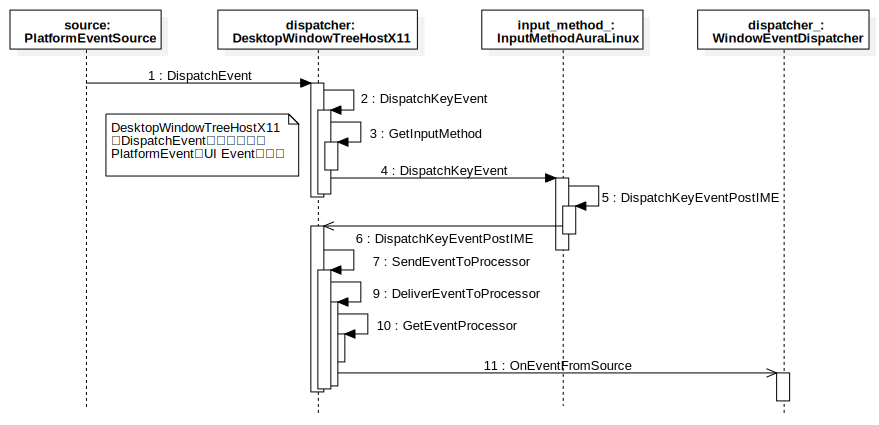
\includegraphics[width=\textwidth]{image/event_study/browser_event_dispatch_sequence_1.pdf} 
  \caption{chromium browser进程事件传递时序图-1} \label{fig:browser_event_dispatch_sequence_1} 
\end{figure}

图~\ref{fig:browser_event_dispatch_sequence_1}
是按键事件从PlatformEventSource到按键分发到特定window之前的调用时序图。

\begin{itemize}
  \item 在第1步调用中(DispatchEvent)就完成了由PlatformEvent到ui::Event的转换。
  也就屏蔽了平台层的事件,转换为chromium内部的事件类型。
  \item DesktopWindowTreeHostX11中的大部分调用都在其父类和祖父类中实现的。
  \item OnEventFromSource函数在WindowEventDispatcher的父类中实现。
\end{itemize}

\begin{spacing}{1.0}
\begin{lstlisting}[language={C++}]
    case KeyPress: {
      ui::KeyEvent keydown_event(xev);
      DispatchKeyEvent(&keydown_event);
      break;
    }
    case KeyRelease: {
      // There is no way to deactivate a window in X11 so ignore input if
      // window is supposed to be 'inactive'. See comments in
      // X11DesktopHandler::DeactivateWindow() for more details.
      if (!IsActive() && !HasCapture())
        break;

      ui::KeyEvent key_event(xev);
      DispatchKeyEvent(&key_event);
      break;
    }
\end{lstlisting}
\end{spacing}

%---------------------------------------------------------------------

\begin{figure}[H] 
  \centering 
  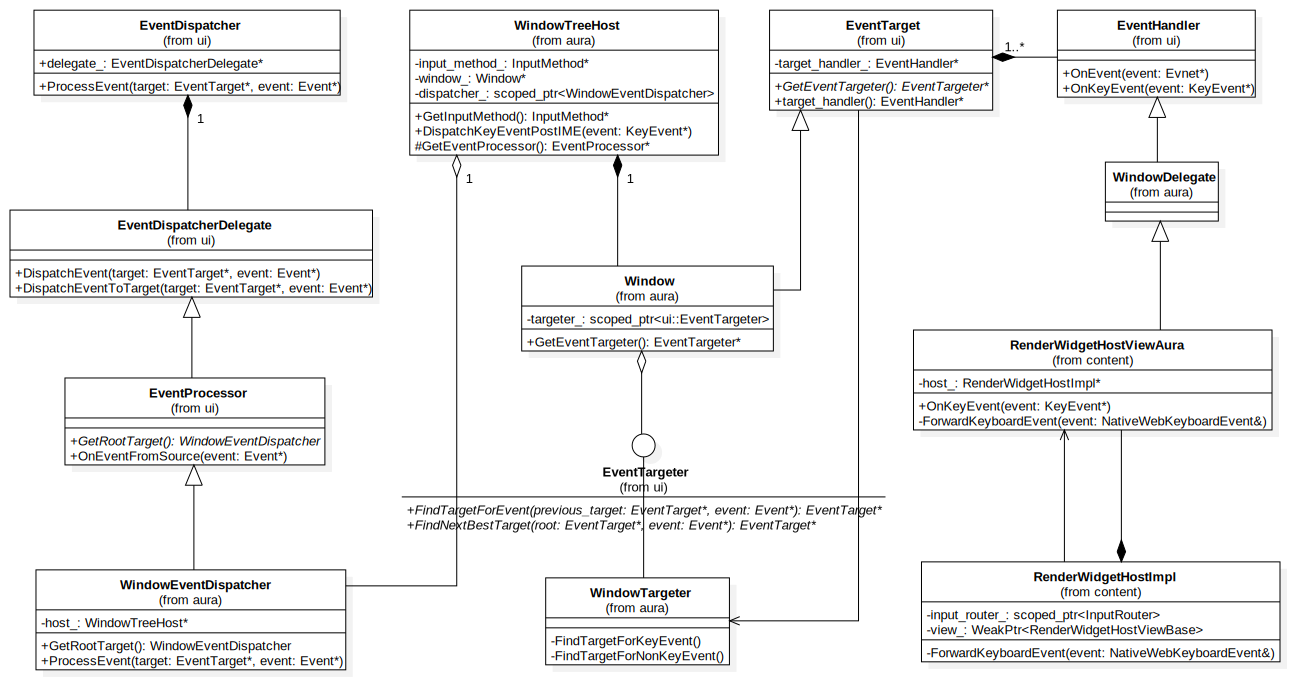
\includegraphics[width=\textwidth]{image/event_study/browser_event_dispatch_class_2.pdf} 
  \caption{chromium browser进程事件传递静态类图-2} \label{fig:linux_event_dispatch_class_2} 
\end{figure}

如图~\ref{fig:linux_event_dispatch_class_2}所示:
是按键事件由UI抽象的EventSource到与Render进程相对应的类RenderWidgetHostImpl之间所涉及的静态类图,其中:
\begin{itemize}
  \item WindowTreeHost继承了EventSource,通过实例化其子类DesktopWindowTreeHostX11来充当UI抽象的事件源。
  \item EventDispatcher和EventDispatcherDelegate是事件分发工作的主要执行者,
  EventDispatcherDelegate类实例化的是其子类WindowEventDispatcher。
  \item window继承自EventTarget可以作为事件的目标,同时又包含EventTargeter对象,用来筛选合适的window处理事件。
  \item EventTarget中实际处理事件的对象是EventHandler。EventTarget中包含3类handler,其中主处理handler仅有一个
  是target\_handler。在主handler处理前会有pre\_target\_list\_中的handler尝试处理事件,
  主handler处理后由post\_target\_list\_尝试处理。这里的处理大部分是指传递给Render进程。
  \item RenderWidgetHostViewAura类继承EventHandler,具有处理事件的能力。通过调试代码发现并不是所有的window内的\\
  target\_handler都是RenderWidgetHostViewAura。
  目前的结论是一个Render进程中的所有window只有一个target\_handler是RenderWidgetHostViewAura。
  \item RenderWidgetHostImpl与Render进程中的RenderWidget对应。
\end{itemize}

\begin{figure}[H] 
  \centering 
  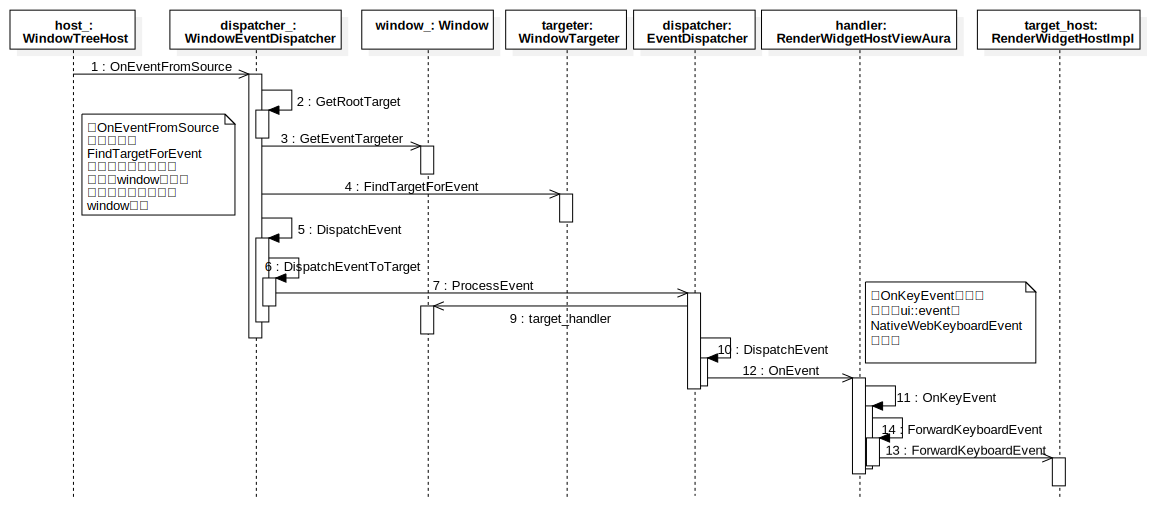
\includegraphics[width=\textwidth]{image/event_study/browser_event_dispatch_sequence_2.pdf} 
  \caption{chromium browser进程事件传递时序图-2} \label{fig:browser_event_dispatch_sequence_2} 
\end{figure}

图~\ref{fig:browser_event_dispatch_sequence_2}
是按键事件从PlatformEventSource到按键分发到特定window之前的调用时序图。

\begin{itemize}
  \item dispatcher\_对象的调用一些方法实现在其父类和祖父类中。
  其中调用GetRootTarget方法返回的对象就是root window。
  \item WindowTargeter类的FindTargetForEvent方法返回合适的window对象作为事件的target。
  由于window是树状结构,处理是会循环调用FindNextBestTarget方法。
  \item RenderWidgetHostViewAura类中的OnKeyEvent方法中完成ui::KeyEvent到NativeWebKeyboardEvent转换,
  NativeWebKeyboardEvent又是blink::WebKeyboardEvent的子类。
  所以按键事件是通过WebKeyboardEvent的形式传递给Render进程的。
\end{itemize}

\begin{spacing}{1.0}
\begin{lstlisting}[language={C++}]
if (!event_to_dispatch->handled())
target = targeter->FindTargetForEvent(root, event_to_dispatch);

EventDispatchDetails details;
while (target) {
details = DispatchEvent(target, event_to_dispatch);

...
  
target = targeter->FindNextBestTarget(target, event_to_dispatch);
}
\end{lstlisting}
\end{spacing}

%---------------------------------------------------------------------

\begin{figure}[H] 
  \centering 
  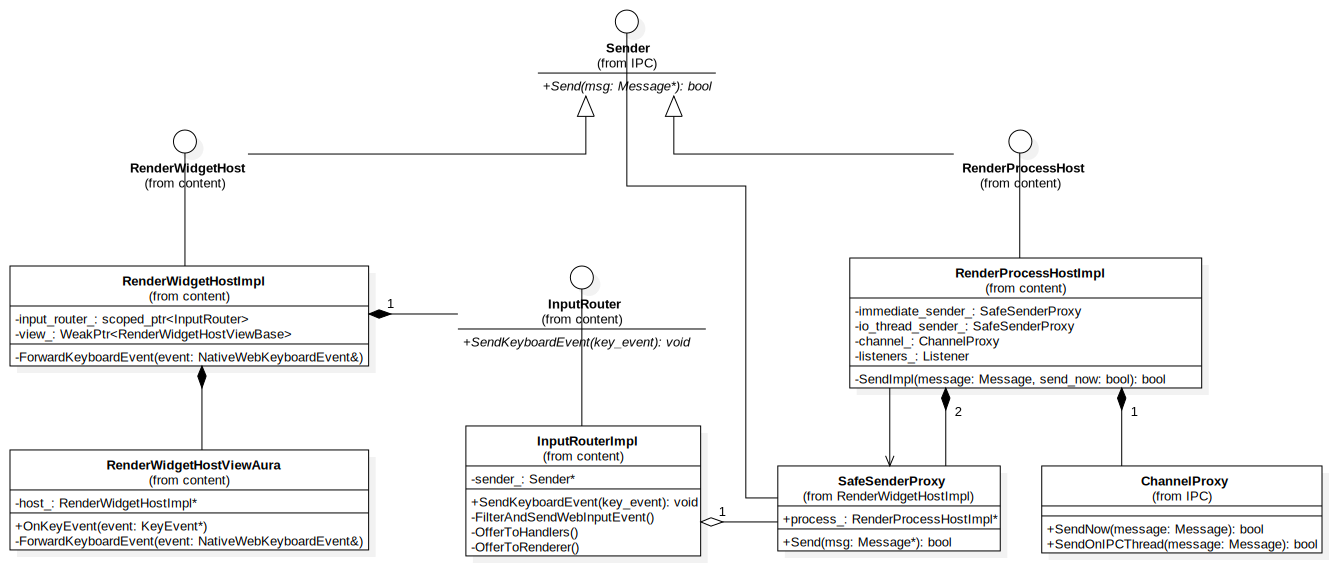
\includegraphics[width=\textwidth]{image/event_study/browser_event_dispatch_class_3.pdf} 
  \caption{chromium browser进程事件传递静态类图-3} \label{fig:browser_event_dispatch_class_3} 
\end{figure}

如图~\ref{fig:browser_event_dispatch_class_3}所示:
是browser进程发送按键消息到render进程过程中涉及的类的静态类图,其中:
\begin{itemize}
  \item RenderWidgetHostImpl、InputRouter、RenderProcessHost等类同时也继承了Listener接口,
  用于接收render进程的消息。
  \item RenderWidgetHost与Render进程中的RenderWidget对应,在chromium给出的多进程框架示意图中可以看出
  一个render进程可以存在多个RenderWidget,但只有一个RenderProcess负责与browser进程通信。
  同样,每个render进程在browser进程中都有一个RenderProcessHost。
  \item 发送消息的具体实施者是ChannelProxy类,在browser进程中实例化的ChannelProxy对象只能发送异步消息,
  后来chromium有在对象内部添加了发送同步消息的函数,但是对外的接口仍默认是异步消息。
  \item 发送消息的底层实现并没有在这里体现,留待后续研究。
\end{itemize}

\newpage
\begin{figure}[H] 
  \centering 
  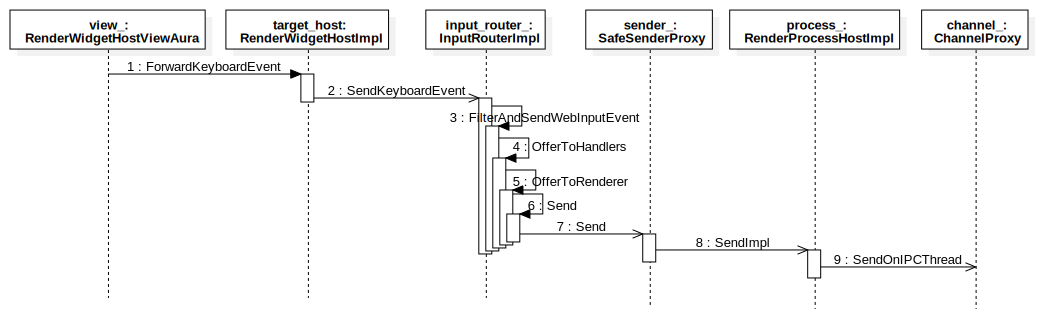
\includegraphics[width=\textwidth]{image/event_study/browser_event_dispatch_sequence_3.pdf} 
  \caption{chromium browser进程事件传递时序图-3} \label{fig:browser_event_dispatch_sequence_3} 
\end{figure}

图~\ref{fig:browser_event_dispatch_sequence_3}
是browser进程发送按键消息到render进程过程中的调用时序图,其中:

\begin{itemize}
  \item SendImpl调用SendOnIPCThread是发送异步消息,同步消息是调用SendNow。
\end{itemize}

\begin{spacing}{1.0}
\begin{lstlisting}[language={C++}]
bool RenderProcessHostImpl::SendImpl(std::unique_ptr<IPC::Message> msg,
                                     bool send_now) {
#if !defined(OS_ANDROID)
  DCHECK(!msg->is_sync());
#endif
  if (!channel_) {
#if defined(OS_ANDROID)
    if (msg->is_sync())
      return false;
#endif
    if (!is_initialized_) {
      queued_messages_.emplace(std::move(msg));
      return true;
    } else {
      return false;
    }
  }

  if (child_process_launcher_.get() && child_process_launcher_->IsStarting()) {
#if defined(OS_ANDROID)
    if (msg->is_sync())
      return false;
#endif
    queued_messages_.emplace(std::move(msg));
    return true;
  }

  if (send_now)
    return channel_->SendNow(std::move(msg));

  return channel_->SendOnIPCThread(std::move(msg));
}
\end{lstlisting}
\end{spacing}

%---------------------------------------------------------------------

\section{按键事件处理流程}
这里的按键事件处理流程指的是render进程接收到按键事件之后的处理流程。
大致过程是从brower进程获取事件;查找事件处理的页面、节点;调用节点注册的监听函数处理事件。

%---------------------------------------------------------------------

\begin{figure}[H] 
  \centering 
  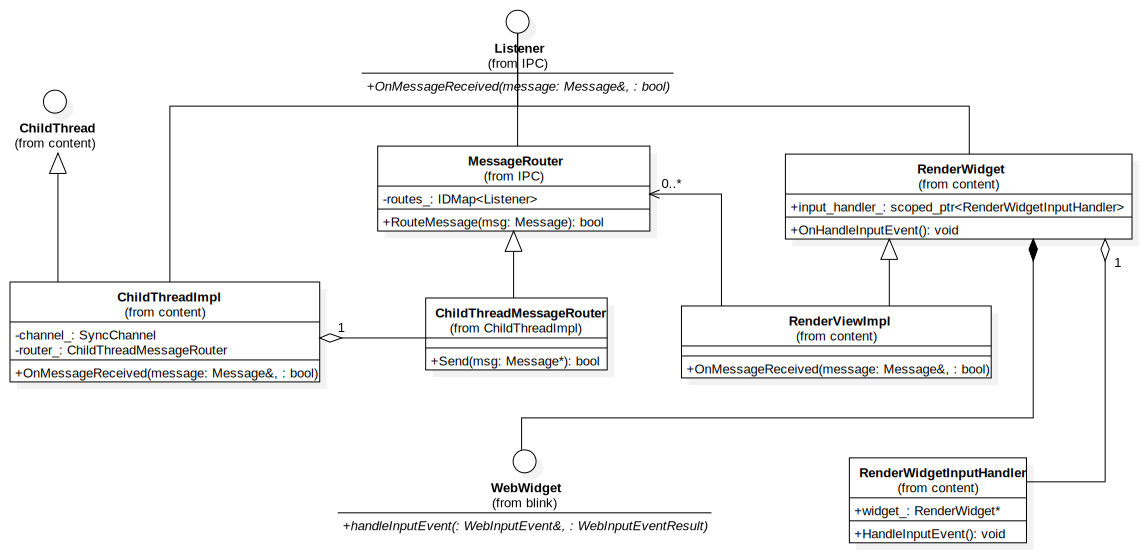
\includegraphics[width=\textwidth]{image/event_study/render_event_dispatch_class.pdf} 
  \caption{chromium render进程处理事件类图-1} \label{fig:render_event_dispatch_class} 
\end{figure}

如图~\ref{fig:render_event_dispatch_class}所示:
是browser进程的按键消息到达render进程后的,到传递给render进程中的特定WebView处理之前所涉及的类的静态类图。其中:
\begin{itemize}
  \item ChildThread、MessageRouter、RenderWidget等类同时也继承了Sender接口,用于发送消息到其他进程。
  \item 消息最先到达ChildThread的OnMessageReceived函数,在这里会处理一些消息,
  剩余消息交于ChildThreadMessageRouter处理。MessageRouter将事件传递给RenderViewImpl处理,
  RenderViewImpl也会处理一些消息,其余交于其父类RenderWidget处理,按键事件最终会传递给RenderWidget。
  \item ChildThreadImpl中的channel实例是SyncChannel对象,可以发送同步消息。
  \item 接收消息的底层实现并没有在这里体现,留待后续研究。
\end{itemize}

\newpage
\begin{figure}[H] 
  \centering 
  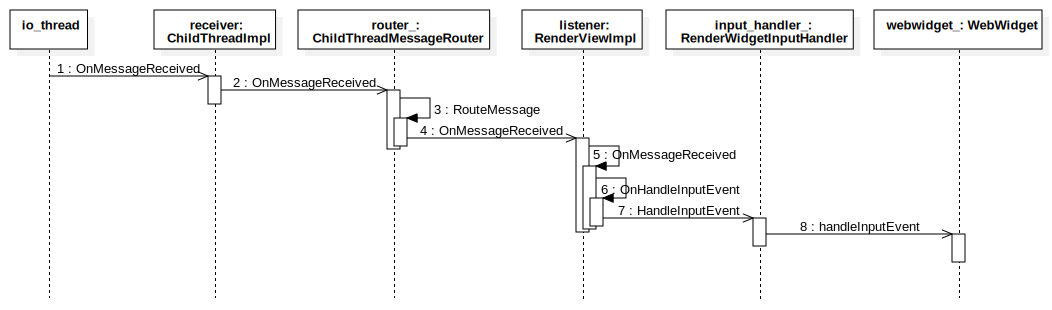
\includegraphics[width=\textwidth]{image/event_study/render_event_dispatch_sequence.pdf} 
  \caption{chromium render进程处理事件时序图-1} \label{fig:render_event_dispatch_sequence} 
\end{figure}

图~\ref{fig:render_event_dispatch_sequence}
是browser进程的按键消息到达render进程后的,到传递给render进程中的特定WebView处理之前的调用时序图,其中:

\begin{itemize}
  \item 在MessageRouter中的RouteMessage中选择哪个RenderView处理事件。
  \item RenderWidgetInputHandler调用RenderWidget的接口获取RenderWidget的webwidget\_处理事件。
\end{itemize}

\begin{spacing}{1.0}
\begin{lstlisting}[language={C++}]
bool MessageRouter::RouteMessage(const IPC::Message& msg) {
  IPC::Listener* listener = routes_.Lookup(msg.routing_id());
  if (!listener)
    return false;

  return listener->OnMessageReceived(msg);
}

void RenderWidgetInputHandler::HandleInputEvent(
    const WebInputEvent& input_event,
    const ui::LatencyInfo& latency_info,
    InputEventDispatchType dispatch_type) {
  ...
  
  WebInputEventResult processed = prevent_default
                                      ? WebInputEventResult::HandledSuppressed
                                      : WebInputEventResult::NotHandled;
  if (input_event.type != WebInputEvent::Char || !suppress_next_char_events_) {
    suppress_next_char_events_ = false;
    if (processed == WebInputEventResult::NotHandled && widget_->webwidget())
      processed = widget_->webwidget()->handleInputEvent(input_event);
  }
  ...  
}
\end{lstlisting}
\end{spacing}

%---------------------------------------------------------------------

\begin{figure}[H] 
  \centering 
  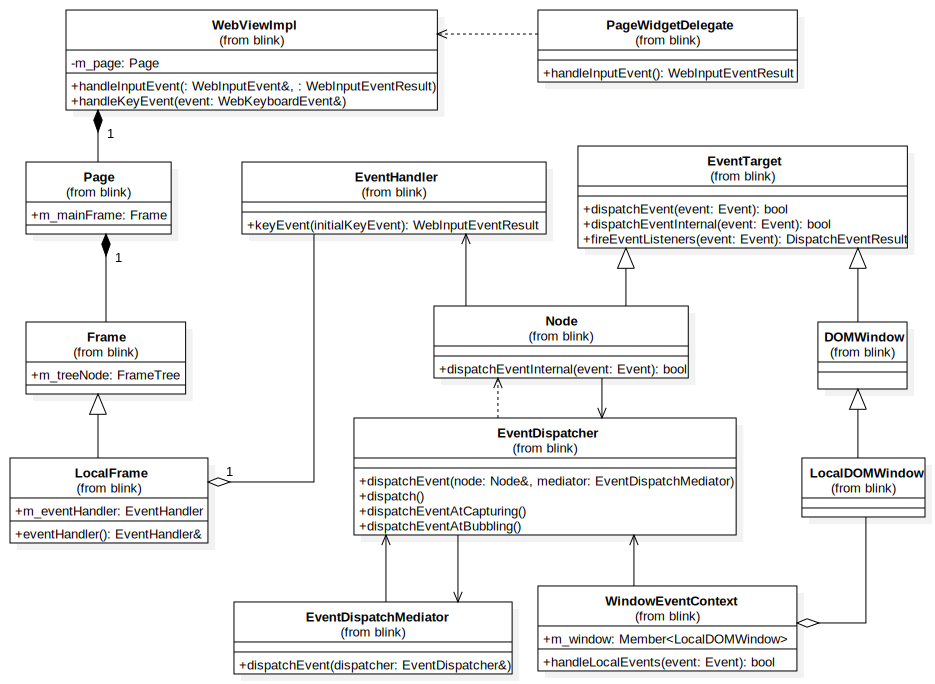
\includegraphics[width=\textwidth]{image/event_study/render_event_handle_class.pdf} 
  \caption{chromium render进程处理事件类图-2} \label{fig:render_event_handle_class} 
\end{figure}

如图~\ref{fig:render_event_handle_class}所示:
是render进程的渲染引擎blink处理按键事件过程中涉及的类的静态类图。其中:
\begin{itemize}
  \item WebViewImpl实现WebWidget接口和WebView接口功能,是RenderWidget的成员变量。
  传递给它的事件将传递给其成员变量m\_page。
  \item 在一个Page中可能包含多个Frame,Page将选择合适的Frame处理传入的事件。
  事件将交于Frame中的m\_eventHandler变量处理。
  \item 在EventHandler中,将遍历DOM树,查找合适的Node处理事件。
  最终通过Node的父类EventTarget调用所以注册的监听函数。
  \item 此过程使用的类都属于blink命名空间,是原来的WebKit内核代码。
\end{itemize}

\newpage
\begin{figure}[H] 
  \centering 
  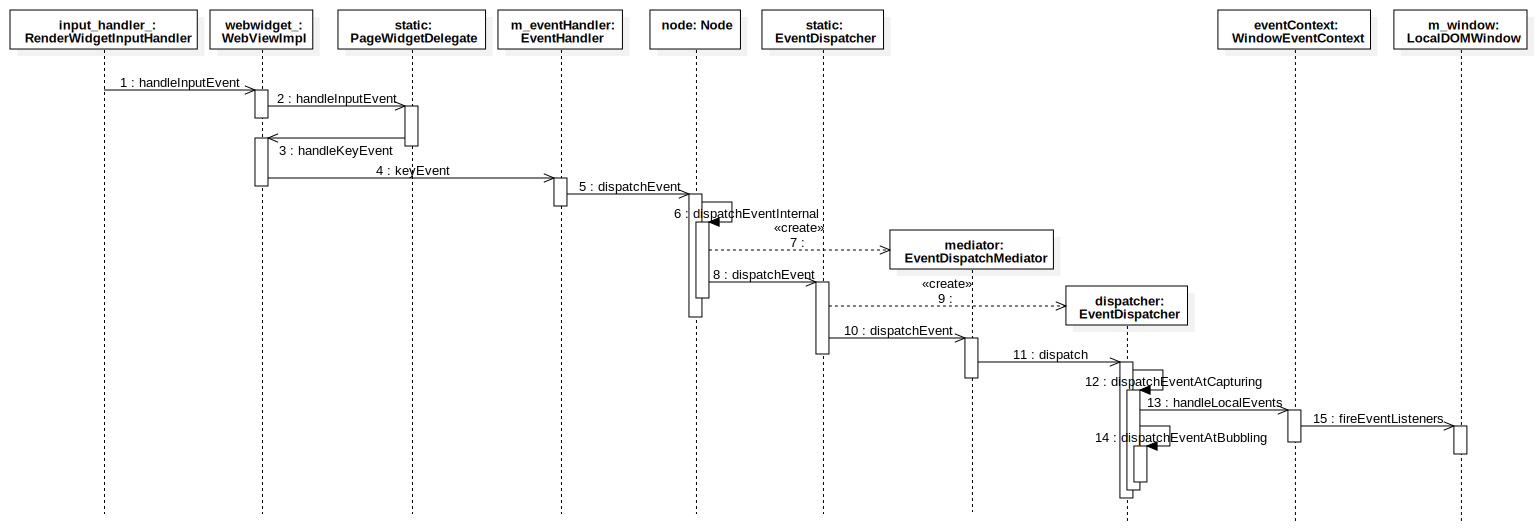
\includegraphics[width=\textwidth]{image/event_study/render_event_handle_sequence.pdf} 
  \caption{chromium render进程处理事件时序图-2} \label{fig:render_event_handle_sequence} 
\end{figure}

图~\ref{fig:render_event_handle_sequence}
是render进程的渲染引擎blink处理按键事件流程调用时序图,其中:
\begin{itemize}
  \item 第3步handleKeyEvent在调用keyEvent方法处理后,若无处理将调用keyEventDefault进行事件的默认处理。
  \item 第4步keyEvent方法中将调用eventTargetNodeForDocument函数,用来查找合适的Node来处理事件。
  \item 第11步EventDispatcher的dispatch方法中首先调用dispatchEventAtCapturing进行事件捕获,
  然后调用dispatchEventAtBubbling进行事件冒泡,这些过程中都会检查事件是否要继续处理。
\end{itemize}

\begin{spacing}{1.0}
\begin{lstlisting}[language={C++}]
DispatchEventResult EventDispatcher::dispatch()
{
    ...
    
    EventDispatchHandlingState* preDispatchEventHandlerResult = nullptr;
    if (dispatchEventPreProcess(preDispatchEventHandlerResult) == ContinueDispatching) {
        if (dispatchEventAtCapturing() == ContinueDispatching) {
            if (dispatchEventAtTarget() == ContinueDispatching)
                dispatchEventAtBubbling();
        }
    }
    
    ...
    return EventTarget::dispatchEventResult(*m_event);
}
\end{lstlisting}
\end{spacing}

%---------------------------------------------------------------------

\ifx\withtbrowser\undefined
\else
\section{引言}
众所周知,chromium是多线程框架的,整个chromium浏览器包括四类进程:browser主进程、render渲染进程、GPU进程和插件进程。
本文所要讲述的chromium事件处理流程主要牵涉到其中的两种进程:browser进程和render进程。

事件处理的大体流程是由browser进程接收并传递给render进程处理。
然而我们知道render会不止一个,那么browser进程如何获取事件?
又如何传递给特定的render进程?render进程如何处理事件消息?我们下面就通过分析代码来一一探明。

chromium系统有多个平台的实现,而每个平台都有自己不同的事件管理方式,chromium也会有一些平台相关的代码。
本文目前主要是研究Linux平台相关的实现,其他平台后续再做研究。
chromium中的事件也有许多类型,如按键事件、鼠标事件、滚轮事件等等。
本文也只是以按键事件为例研究,在以下内容中,如无特殊说明,事件均指的是按键事件。

\section{按键事件获取流程}
\begin{figure}[H] 
  \centering 
  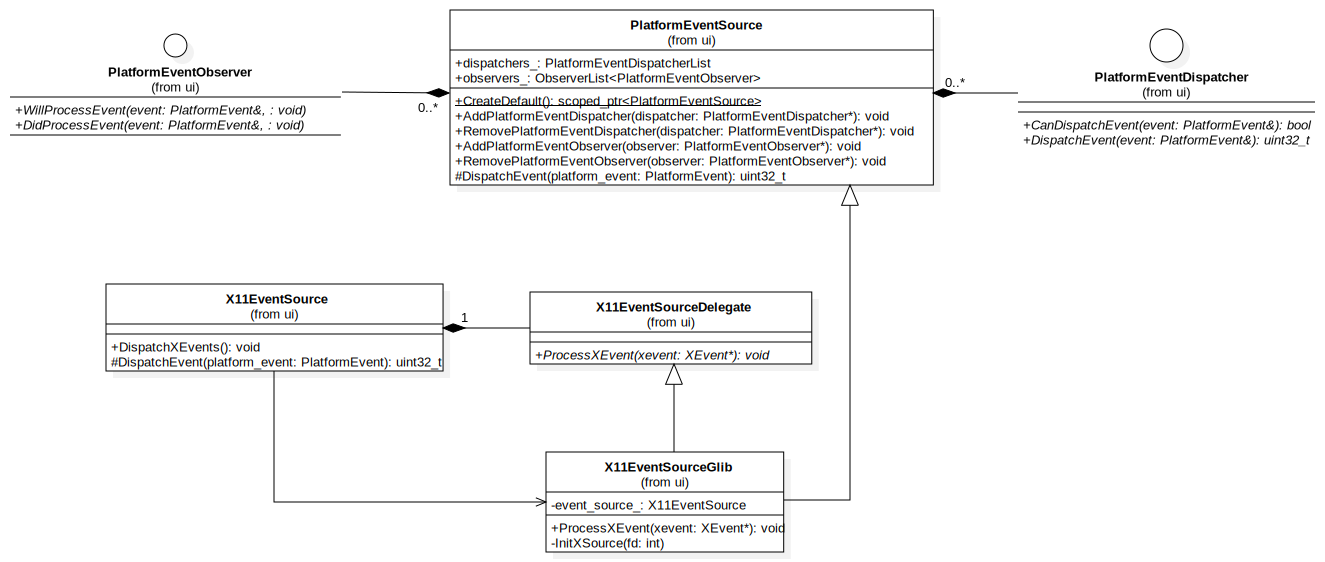
\includegraphics[width=\textwidth]{image/event_study/linux_event_source_class.pdf} 
  \caption{chromium linux平台事件源静态类图} \label{fig:linux_event_source_class} 
\end{figure}

如第图~\ref{fig:linux_event_source_class}所示:
chromium对事件源抽象了一个PlatformEventSource类表示,不同的平台继承该类实现自己平台的子类。
不过,目前发现仅有Linux平台实现了其子类X11EventSource与X11EventSourceGlib。
Windows和Android都未采用该方法。

\begin{figure}[H] 
  \centering 
  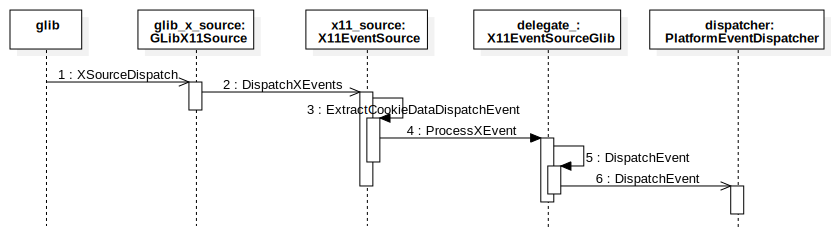
\includegraphics[width=\textwidth]{image/event_study/linux_get_event_from_source.pdf} 
  \caption{chromium linux平台事件获取时序图} \label{fig:linux_get_event_from_source} 
\end{figure}

browser进程获取按键事件的调用时序图如图~\ref{fig:linux_get_event_from_source}所示:
\begin{itemize}
  \item 在browser进程启动时,会创建一个线程循环调用g\_main\_context\_iteration方法。其作用是驱动glib检查事件,如果有事件发生,则glib会调用初始化时注册的XSourceDispatch回调来将事件传递给PlatformEventSource的子类。
  \item 第5步调用时是调用的父类PlatformEventSource方法,将事件传递给PlatformEventDispatcher。
\end{itemize}

\begin{spacing}{1.0}
\begin{lstlisting}[language={C++}]
  for (;;) {
    // Don't block if we think we have more work to do.
    bool block = !more_work_is_plausible;

    more_work_is_plausible = g_main_context_iteration(context_, block);
    if (state_->should_quit)
      break;

    more_work_is_plausible |= state_->delegate->DoWork();
    if (state_->should_quit)
      break;

    more_work_is_plausible |=
        state_->delegate->DoDelayedWork(&delayed_work_time_);
    if (state_->should_quit)
      break;

    if (more_work_is_plausible)
      continue;

    more_work_is_plausible = state_->delegate->DoIdleWork();
    if (state_->should_quit)
      break;
  }
\end{lstlisting}
\end{spacing}

\section{按键事件传递流程}
这里的按键传递流程是指browser进程从事件源处取得事件之后将其传递给特定的render进程的过程。
这里研究的是使用chromium的aura窗口系统的流程,平台是Linux平台,
然而据初步研究Windows和Android也是使用同样的流程,只是传入事件的位置不同罢了。

%---------------------------------------------------------------------

\begin{figure}[H] 
  \centering 
  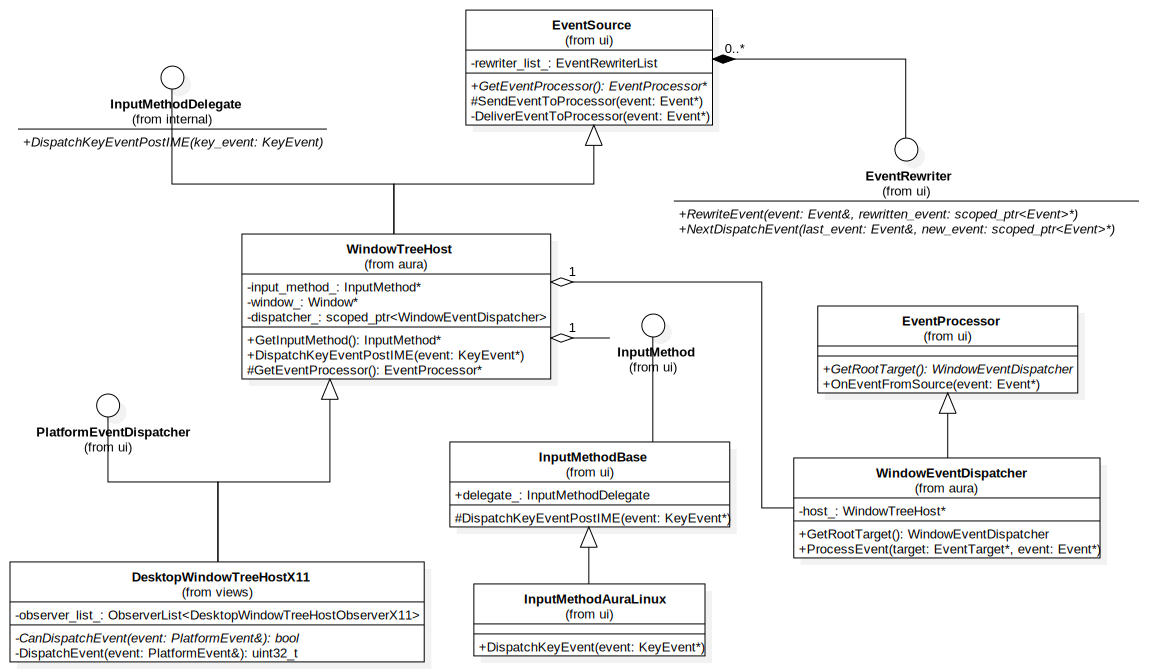
\includegraphics[width=\textwidth]{image/event_study/browser_event_dispatch_class_1.pdf} 
  \caption{chromium browser进程事件传递静态类图-1} \label{fig:linux_event_dispatch_class_1} 
\end{figure}

图~\ref{fig:linux_event_dispatch_class_1}是按键事件从PlatformEventSource到按键分发到特定window之前,
所涉及的主要类的静态类图。
\begin{itemize}
  \item DesktopWindowTreeHostX11类实现PlatformEventDispatcher接口,同时又继承了WindowTreeHost和EventSource。
  这样DesktopWindowTreeHostX11类在broeser进程中就扮演了重要的角色,可谓身兼数职。
  在事件处理流程上看它既是PlatformEventSource的dispatcher,又是UI系统的EventSource。
  \item EventSource中包含EventRewriter对象,可以在事件处理前改写事件。
  \item InputMethodBase内存在WindowTreeHost的引用。
\end{itemize}

\begin{figure}[H] 
  \centering 
  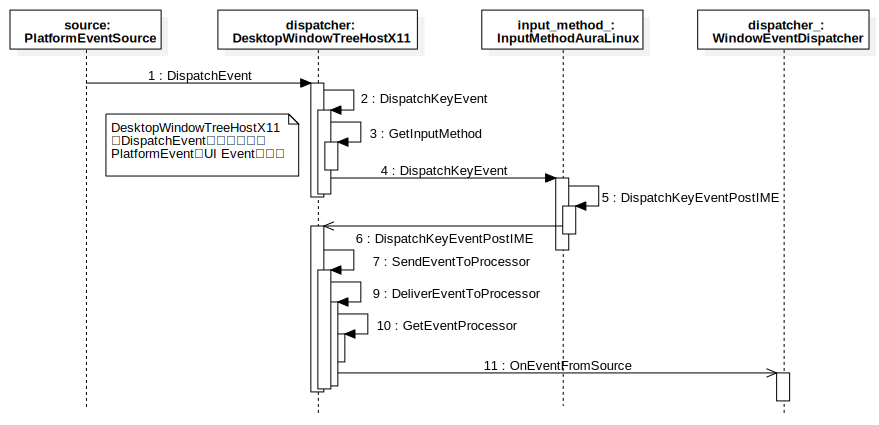
\includegraphics[width=\textwidth]{image/event_study/browser_event_dispatch_sequence_1.pdf} 
  \caption{chromium browser进程事件传递时序图-1} \label{fig:browser_event_dispatch_sequence_1} 
\end{figure}

图~\ref{fig:browser_event_dispatch_sequence_1}
是按键事件从PlatformEventSource到按键分发到特定window之前的调用时序图。

\begin{itemize}
  \item 在第1步调用中(DispatchEvent)就完成了由PlatformEvent到ui::Event的转换。
  也就屏蔽了平台层的事件,转换为chromium内部的事件类型。
  \item DesktopWindowTreeHostX11中的大部分调用都在其父类和祖父类中实现的。
  \item OnEventFromSource函数在WindowEventDispatcher的父类中实现。
\end{itemize}

\begin{spacing}{1.0}
\begin{lstlisting}[language={C++}]
    case KeyPress: {
      ui::KeyEvent keydown_event(xev);
      DispatchKeyEvent(&keydown_event);
      break;
    }
    case KeyRelease: {
      // There is no way to deactivate a window in X11 so ignore input if
      // window is supposed to be 'inactive'. See comments in
      // X11DesktopHandler::DeactivateWindow() for more details.
      if (!IsActive() && !HasCapture())
        break;

      ui::KeyEvent key_event(xev);
      DispatchKeyEvent(&key_event);
      break;
    }
\end{lstlisting}
\end{spacing}

%---------------------------------------------------------------------

\begin{figure}[H] 
  \centering 
  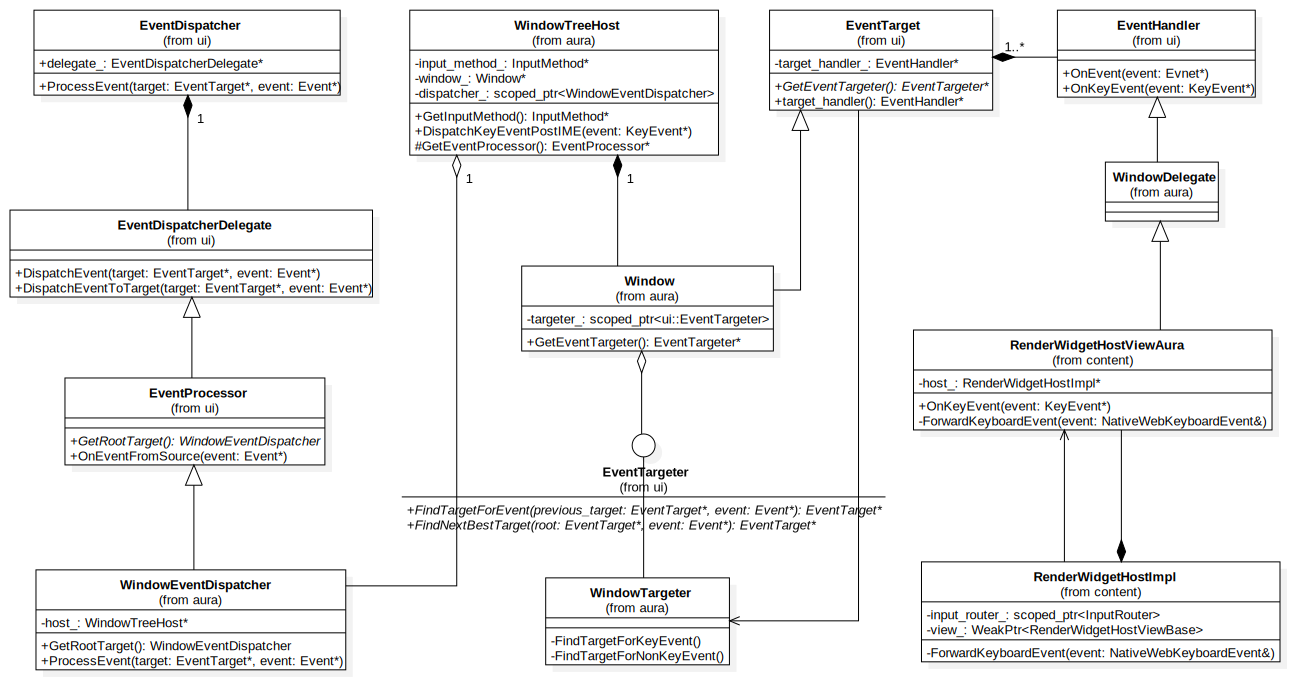
\includegraphics[width=\textwidth]{image/event_study/browser_event_dispatch_class_2.pdf} 
  \caption{chromium browser进程事件传递静态类图-2} \label{fig:linux_event_dispatch_class_2} 
\end{figure}

如图~\ref{fig:linux_event_dispatch_class_2}所示:
是按键事件由UI抽象的EventSource到与Render进程相对应的类RenderWidgetHostImpl之间所涉及的静态类图,其中:
\begin{itemize}
  \item WindowTreeHost继承了EventSource,通过实例化其子类DesktopWindowTreeHostX11来充当UI抽象的事件源。
  \item EventDispatcher和EventDispatcherDelegate是事件分发工作的主要执行者,
  EventDispatcherDelegate类实例化的是其子类WindowEventDispatcher。
  \item window继承自EventTarget可以作为事件的目标,同时又包含EventTargeter对象,用来筛选合适的window处理事件。
  \item EventTarget中实际处理事件的对象是EventHandler。EventTarget中包含3类handler,其中主处理handler仅有一个
  是target\_handler。在主handler处理前会有pre\_target\_list\_中的handler尝试处理事件,
  主handler处理后由post\_target\_list\_尝试处理。这里的处理大部分是指传递给Render进程。
  \item RenderWidgetHostViewAura类继承EventHandler,具有处理事件的能力。通过调试代码发现并不是所有的window内的\\
  target\_handler都是RenderWidgetHostViewAura。
  目前的结论是一个Render进程中的所有window只有一个target\_handler是RenderWidgetHostViewAura。
  \item RenderWidgetHostImpl与Render进程中的RenderWidget对应。
\end{itemize}

\begin{figure}[H] 
  \centering 
  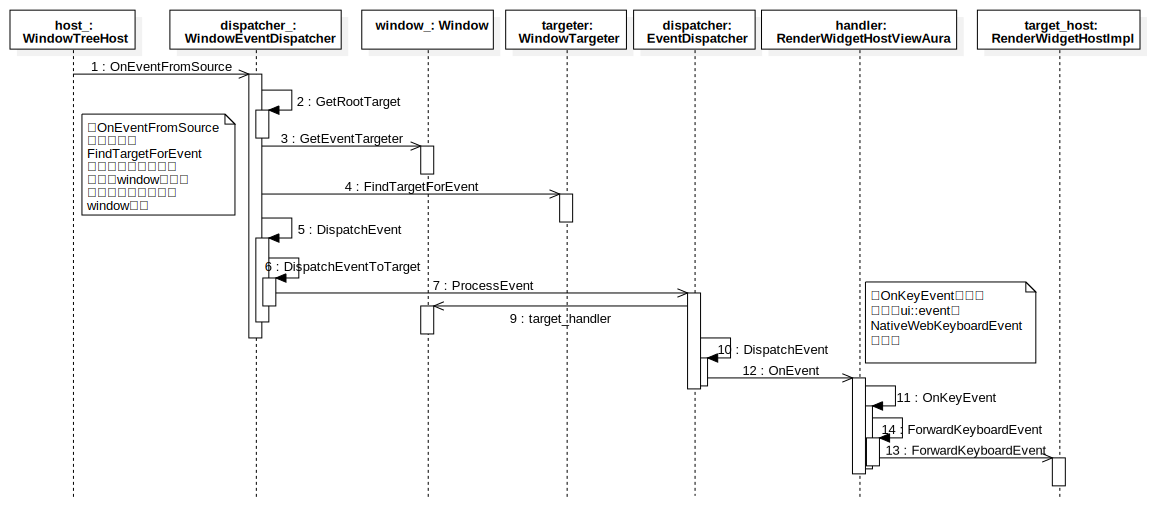
\includegraphics[width=\textwidth]{image/event_study/browser_event_dispatch_sequence_2.pdf} 
  \caption{chromium browser进程事件传递时序图-2} \label{fig:browser_event_dispatch_sequence_2} 
\end{figure}

图~\ref{fig:browser_event_dispatch_sequence_2}
是按键事件从PlatformEventSource到按键分发到特定window之前的调用时序图。

\begin{itemize}
  \item dispatcher\_对象的调用一些方法实现在其父类和祖父类中。
  其中调用GetRootTarget方法返回的对象就是root window。
  \item WindowTargeter类的FindTargetForEvent方法返回合适的window对象作为事件的target。
  由于window是树状结构,处理是会循环调用FindNextBestTarget方法。
  \item RenderWidgetHostViewAura类中的OnKeyEvent方法中完成ui::KeyEvent到NativeWebKeyboardEvent转换,
  NativeWebKeyboardEvent又是blink::WebKeyboardEvent的子类。
  所以按键事件是通过WebKeyboardEvent的形式传递给Render进程的。
\end{itemize}

\begin{spacing}{1.0}
\begin{lstlisting}[language={C++}]
if (!event_to_dispatch->handled())
target = targeter->FindTargetForEvent(root, event_to_dispatch);

EventDispatchDetails details;
while (target) {
details = DispatchEvent(target, event_to_dispatch);

...
  
target = targeter->FindNextBestTarget(target, event_to_dispatch);
}
\end{lstlisting}
\end{spacing}

%---------------------------------------------------------------------

\begin{figure}[H] 
  \centering 
  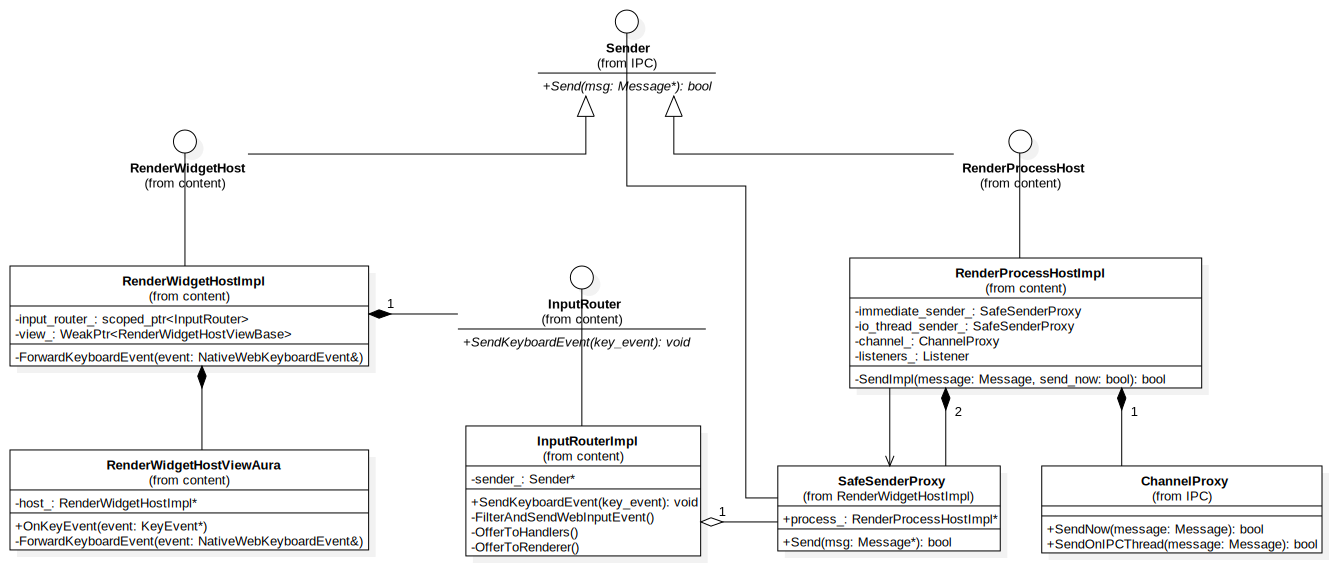
\includegraphics[width=\textwidth]{image/event_study/browser_event_dispatch_class_3.pdf} 
  \caption{chromium browser进程事件传递静态类图-3} \label{fig:browser_event_dispatch_class_3} 
\end{figure}

如图~\ref{fig:browser_event_dispatch_class_3}所示:
是browser进程发送按键消息到render进程过程中涉及的类的静态类图,其中:
\begin{itemize}
  \item RenderWidgetHostImpl、InputRouter、RenderProcessHost等类同时也继承了Listener接口,
  用于接收render进程的消息。
  \item RenderWidgetHost与Render进程中的RenderWidget对应,在chromium给出的多进程框架示意图中可以看出
  一个render进程可以存在多个RenderWidget,但只有一个RenderProcess负责与browser进程通信。
  同样,每个render进程在browser进程中都有一个RenderProcessHost。
  \item 发送消息的具体实施者是ChannelProxy类,在browser进程中实例化的ChannelProxy对象只能发送异步消息,
  后来chromium有在对象内部添加了发送同步消息的函数,但是对外的接口仍默认是异步消息。
  \item 发送消息的底层实现并没有在这里体现,留待后续研究。
\end{itemize}

\newpage
\begin{figure}[H] 
  \centering 
  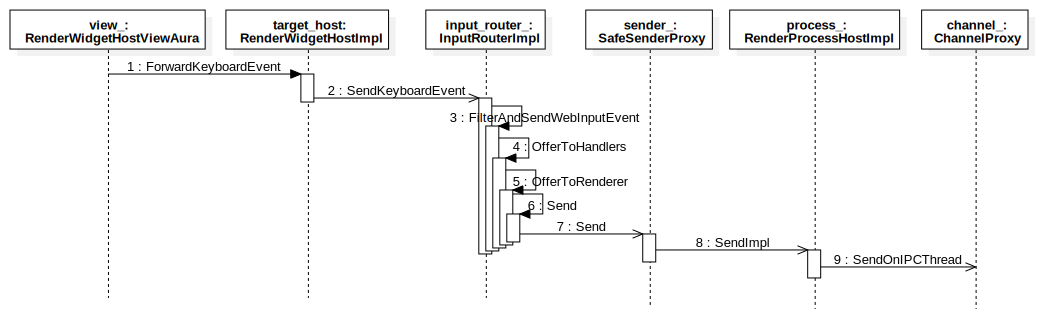
\includegraphics[width=\textwidth]{image/event_study/browser_event_dispatch_sequence_3.pdf} 
  \caption{chromium browser进程事件传递时序图-3} \label{fig:browser_event_dispatch_sequence_3} 
\end{figure}

图~\ref{fig:browser_event_dispatch_sequence_3}
是browser进程发送按键消息到render进程过程中的调用时序图,其中:

\begin{itemize}
  \item SendImpl调用SendOnIPCThread是发送异步消息,同步消息是调用SendNow。
\end{itemize}

\begin{spacing}{1.0}
\begin{lstlisting}[language={C++}]
bool RenderProcessHostImpl::SendImpl(std::unique_ptr<IPC::Message> msg,
                                     bool send_now) {
#if !defined(OS_ANDROID)
  DCHECK(!msg->is_sync());
#endif
  if (!channel_) {
#if defined(OS_ANDROID)
    if (msg->is_sync())
      return false;
#endif
    if (!is_initialized_) {
      queued_messages_.emplace(std::move(msg));
      return true;
    } else {
      return false;
    }
  }

  if (child_process_launcher_.get() && child_process_launcher_->IsStarting()) {
#if defined(OS_ANDROID)
    if (msg->is_sync())
      return false;
#endif
    queued_messages_.emplace(std::move(msg));
    return true;
  }

  if (send_now)
    return channel_->SendNow(std::move(msg));

  return channel_->SendOnIPCThread(std::move(msg));
}
\end{lstlisting}
\end{spacing}

%---------------------------------------------------------------------

\section{按键事件处理流程}
这里的按键事件处理流程指的是render进程接收到按键事件之后的处理流程。
大致过程是从brower进程获取事件;查找事件处理的页面、节点;调用节点注册的监听函数处理事件。

%---------------------------------------------------------------------

\begin{figure}[H] 
  \centering 
  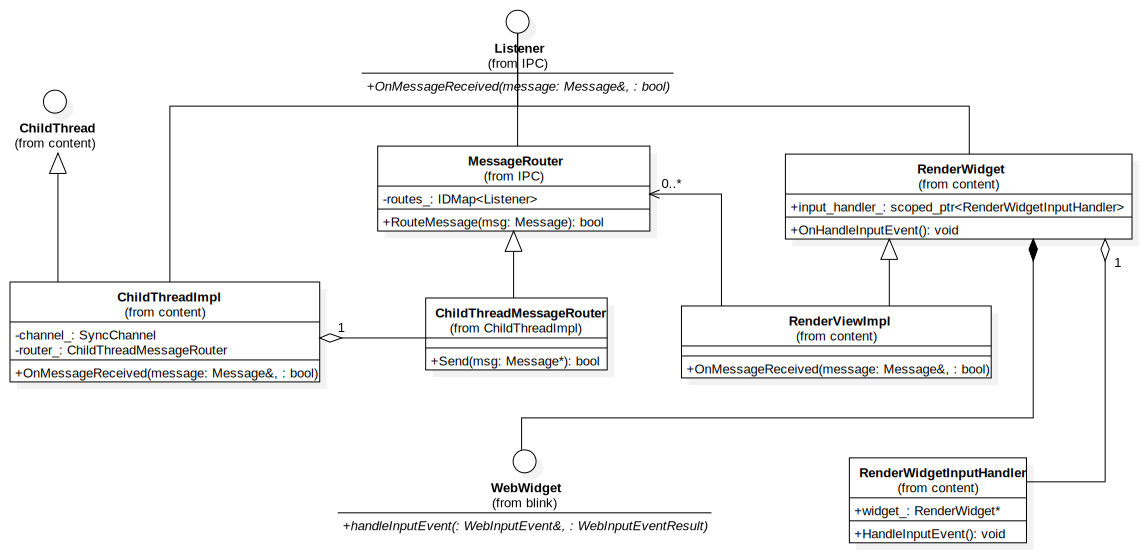
\includegraphics[width=\textwidth]{image/event_study/render_event_dispatch_class.pdf} 
  \caption{chromium render进程处理事件类图-1} \label{fig:render_event_dispatch_class} 
\end{figure}

如图~\ref{fig:render_event_dispatch_class}所示:
是browser进程的按键消息到达render进程后的,到传递给render进程中的特定WebView处理之前所涉及的类的静态类图。其中:
\begin{itemize}
  \item ChildThread、MessageRouter、RenderWidget等类同时也继承了Sender接口,用于发送消息到其他进程。
  \item 消息最先到达ChildThread的OnMessageReceived函数,在这里会处理一些消息,
  剩余消息交于ChildThreadMessageRouter处理。MessageRouter将事件传递给RenderViewImpl处理,
  RenderViewImpl也会处理一些消息,其余交于其父类RenderWidget处理,按键事件最终会传递给RenderWidget。
  \item ChildThreadImpl中的channel实例是SyncChannel对象,可以发送同步消息。
  \item 接收消息的底层实现并没有在这里体现,留待后续研究。
\end{itemize}

\newpage
\begin{figure}[H] 
  \centering 
  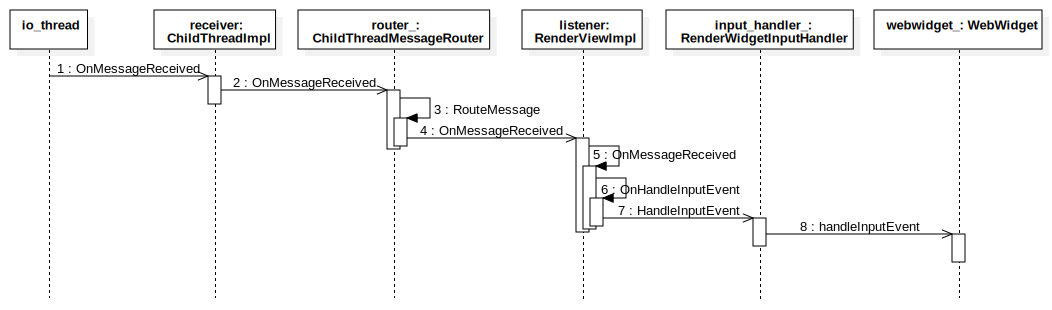
\includegraphics[width=\textwidth]{image/event_study/render_event_dispatch_sequence.pdf} 
  \caption{chromium render进程处理事件时序图-1} \label{fig:render_event_dispatch_sequence} 
\end{figure}

图~\ref{fig:render_event_dispatch_sequence}
是browser进程的按键消息到达render进程后的,到传递给render进程中的特定WebView处理之前的调用时序图,其中:

\begin{itemize}
  \item 在MessageRouter中的RouteMessage中选择哪个RenderView处理事件。
  \item RenderWidgetInputHandler调用RenderWidget的接口获取RenderWidget的webwidget\_处理事件。
\end{itemize}

\begin{spacing}{1.0}
\begin{lstlisting}[language={C++}]
bool MessageRouter::RouteMessage(const IPC::Message& msg) {
  IPC::Listener* listener = routes_.Lookup(msg.routing_id());
  if (!listener)
    return false;

  return listener->OnMessageReceived(msg);
}

void RenderWidgetInputHandler::HandleInputEvent(
    const WebInputEvent& input_event,
    const ui::LatencyInfo& latency_info,
    InputEventDispatchType dispatch_type) {
  ...
  
  WebInputEventResult processed = prevent_default
                                      ? WebInputEventResult::HandledSuppressed
                                      : WebInputEventResult::NotHandled;
  if (input_event.type != WebInputEvent::Char || !suppress_next_char_events_) {
    suppress_next_char_events_ = false;
    if (processed == WebInputEventResult::NotHandled && widget_->webwidget())
      processed = widget_->webwidget()->handleInputEvent(input_event);
  }
  ...  
}
\end{lstlisting}
\end{spacing}

%---------------------------------------------------------------------

\begin{figure}[H] 
  \centering 
  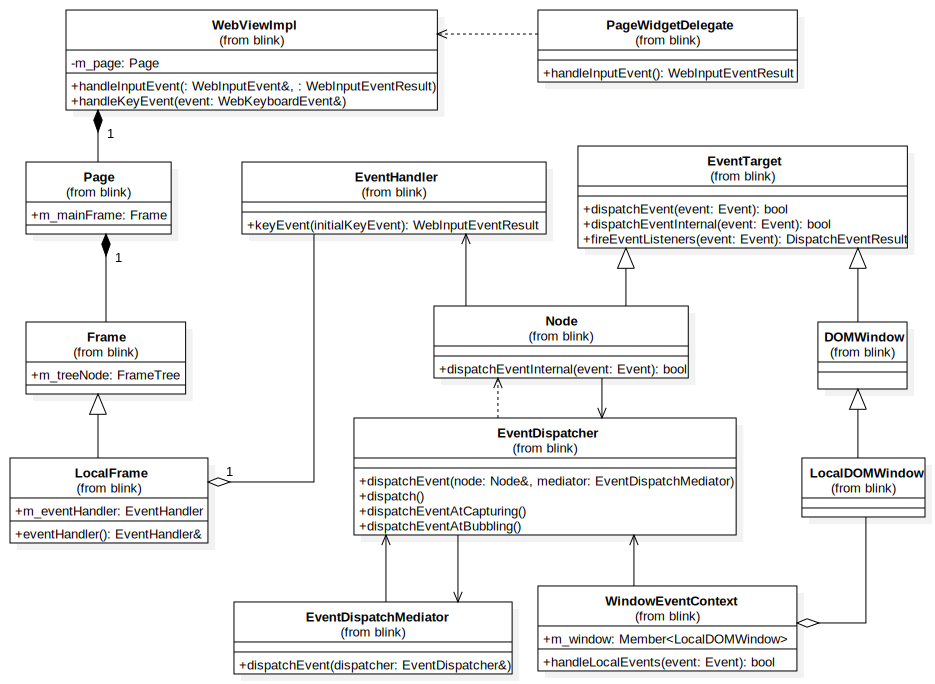
\includegraphics[width=\textwidth]{image/event_study/render_event_handle_class.pdf} 
  \caption{chromium render进程处理事件类图-2} \label{fig:render_event_handle_class} 
\end{figure}

如图~\ref{fig:render_event_handle_class}所示:
是render进程的渲染引擎blink处理按键事件过程中涉及的类的静态类图。其中:
\begin{itemize}
  \item WebViewImpl实现WebWidget接口和WebView接口功能,是RenderWidget的成员变量。
  传递给它的事件将传递给其成员变量m\_page。
  \item 在一个Page中可能包含多个Frame,Page将选择合适的Frame处理传入的事件。
  事件将交于Frame中的m\_eventHandler变量处理。
  \item 在EventHandler中,将遍历DOM树,查找合适的Node处理事件。
  最终通过Node的父类EventTarget调用所以注册的监听函数。
  \item 此过程使用的类都属于blink命名空间,是原来的WebKit内核代码。
\end{itemize}

\newpage
\begin{figure}[H] 
  \centering 
  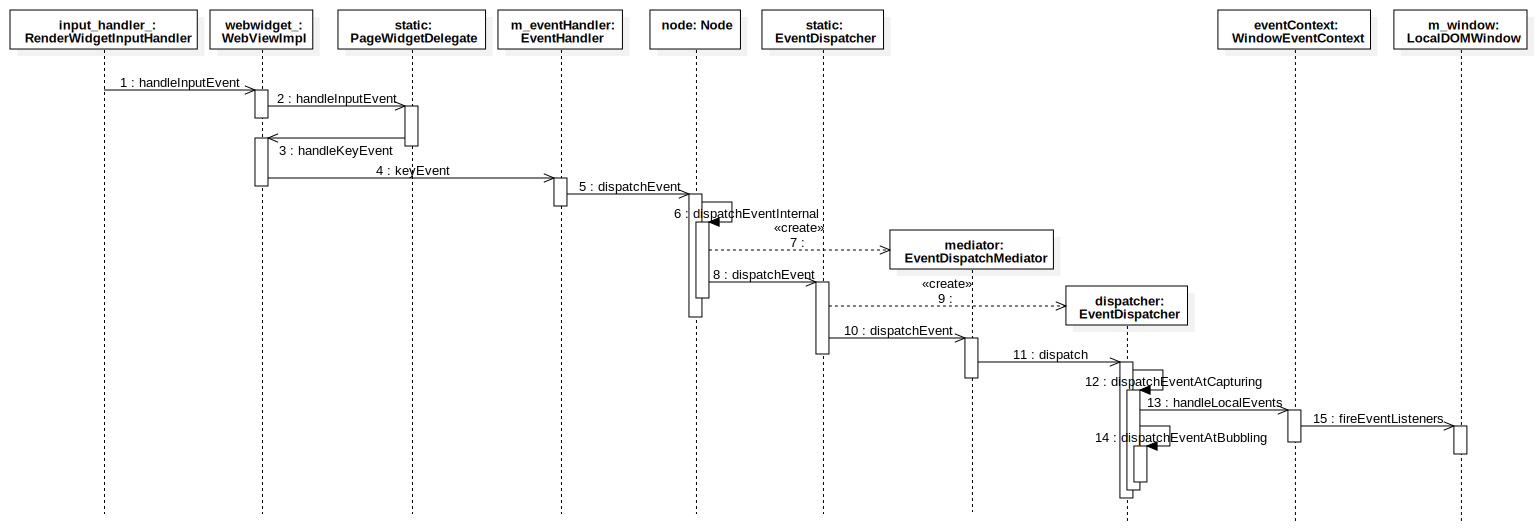
\includegraphics[width=\textwidth]{image/event_study/render_event_handle_sequence.pdf} 
  \caption{chromium render进程处理事件时序图-2} \label{fig:render_event_handle_sequence} 
\end{figure}

图~\ref{fig:render_event_handle_sequence}
是render进程的渲染引擎blink处理按键事件流程调用时序图,其中:
\begin{itemize}
  \item 第3步handleKeyEvent在调用keyEvent方法处理后,若无处理将调用keyEventDefault进行事件的默认处理。
  \item 第4步keyEvent方法中将调用eventTargetNodeForDocument函数,用来查找合适的Node来处理事件。
  \item 第11步EventDispatcher的dispatch方法中首先调用dispatchEventAtCapturing进行事件捕获,
  然后调用dispatchEventAtBubbling进行事件冒泡,这些过程中都会检查事件是否要继续处理。
\end{itemize}

\begin{spacing}{1.0}
\begin{lstlisting}[language={C++}]
DispatchEventResult EventDispatcher::dispatch()
{
    ...
    
    EventDispatchHandlingState* preDispatchEventHandlerResult = nullptr;
    if (dispatchEventPreProcess(preDispatchEventHandlerResult) == ContinueDispatching) {
        if (dispatchEventAtCapturing() == ContinueDispatching) {
            if (dispatchEventAtTarget() == ContinueDispatching)
                dispatchEventAtBubbling();
        }
    }
    
    ...
    return EventTarget::dispatchEventResult(*m_event);
}
\end{lstlisting}
\end{spacing}

%---------------------------------------------------------------------

\ifx\withtbrowser\undefined
\else
\section{引言}
众所周知,chromium是多线程框架的,整个chromium浏览器包括四类进程:browser主进程、render渲染进程、GPU进程和插件进程。
本文所要讲述的chromium事件处理流程主要牵涉到其中的两种进程:browser进程和render进程。

事件处理的大体流程是由browser进程接收并传递给render进程处理。
然而我们知道render会不止一个,那么browser进程如何获取事件?
又如何传递给特定的render进程?render进程如何处理事件消息?我们下面就通过分析代码来一一探明。

chromium系统有多个平台的实现,而每个平台都有自己不同的事件管理方式,chromium也会有一些平台相关的代码。
本文目前主要是研究Linux平台相关的实现,其他平台后续再做研究。
chromium中的事件也有许多类型,如按键事件、鼠标事件、滚轮事件等等。
本文也只是以按键事件为例研究,在以下内容中,如无特殊说明,事件均指的是按键事件。

\section{按键事件获取流程}
\begin{figure}[H] 
  \centering 
  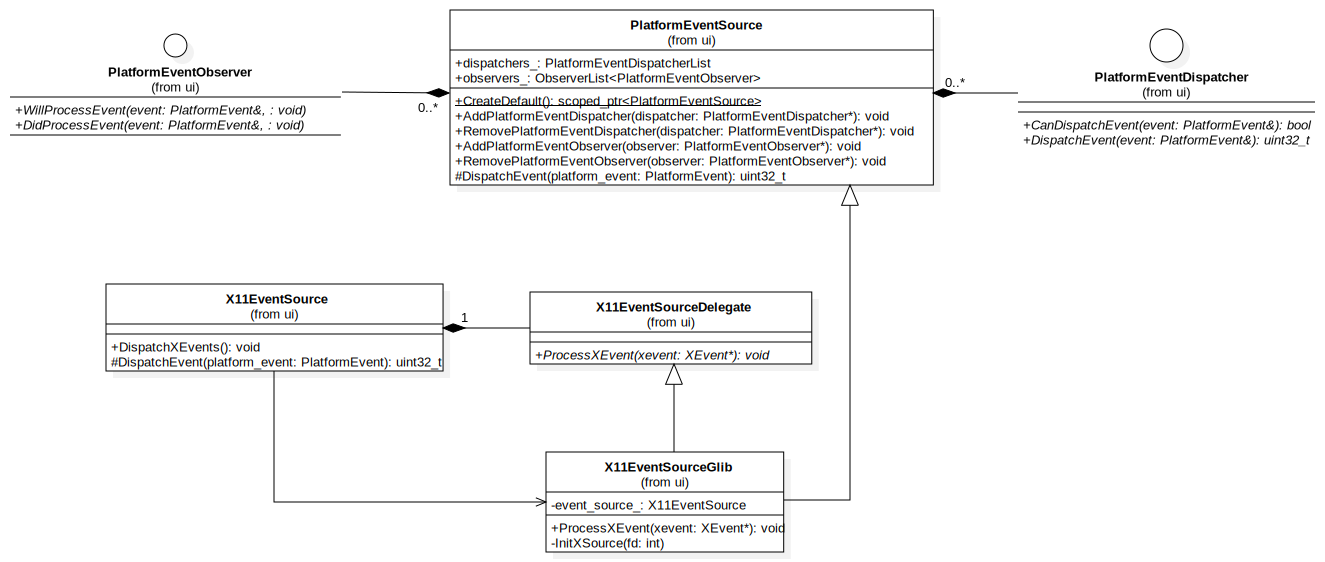
\includegraphics[width=\textwidth]{image/event_study/linux_event_source_class.pdf} 
  \caption{chromium linux平台事件源静态类图} \label{fig:linux_event_source_class} 
\end{figure}

如第图~\ref{fig:linux_event_source_class}所示:
chromium对事件源抽象了一个PlatformEventSource类表示,不同的平台继承该类实现自己平台的子类。
不过,目前发现仅有Linux平台实现了其子类X11EventSource与X11EventSourceGlib。
Windows和Android都未采用该方法。

\begin{figure}[H] 
  \centering 
  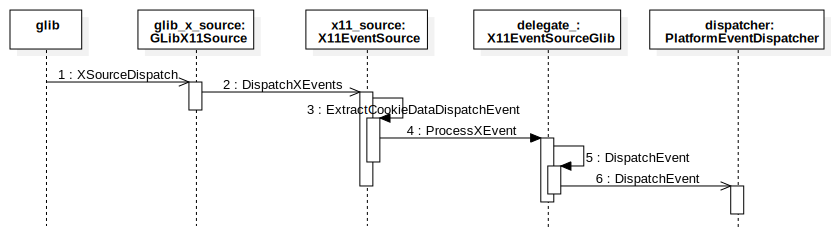
\includegraphics[width=\textwidth]{image/event_study/linux_get_event_from_source.pdf} 
  \caption{chromium linux平台事件获取时序图} \label{fig:linux_get_event_from_source} 
\end{figure}

browser进程获取按键事件的调用时序图如图~\ref{fig:linux_get_event_from_source}所示:
\begin{itemize}
  \item 在browser进程启动时,会创建一个线程循环调用g\_main\_context\_iteration方法。其作用是驱动glib检查事件,如果有事件发生,则glib会调用初始化时注册的XSourceDispatch回调来将事件传递给PlatformEventSource的子类。
  \item 第5步调用时是调用的父类PlatformEventSource方法,将事件传递给PlatformEventDispatcher。
\end{itemize}

\begin{spacing}{1.0}
\begin{lstlisting}[language={C++}]
  for (;;) {
    // Don't block if we think we have more work to do.
    bool block = !more_work_is_plausible;

    more_work_is_plausible = g_main_context_iteration(context_, block);
    if (state_->should_quit)
      break;

    more_work_is_plausible |= state_->delegate->DoWork();
    if (state_->should_quit)
      break;

    more_work_is_plausible |=
        state_->delegate->DoDelayedWork(&delayed_work_time_);
    if (state_->should_quit)
      break;

    if (more_work_is_plausible)
      continue;

    more_work_is_plausible = state_->delegate->DoIdleWork();
    if (state_->should_quit)
      break;
  }
\end{lstlisting}
\end{spacing}

\section{按键事件传递流程}
这里的按键传递流程是指browser进程从事件源处取得事件之后将其传递给特定的render进程的过程。
这里研究的是使用chromium的aura窗口系统的流程,平台是Linux平台,
然而据初步研究Windows和Android也是使用同样的流程,只是传入事件的位置不同罢了。

%---------------------------------------------------------------------

\begin{figure}[H] 
  \centering 
  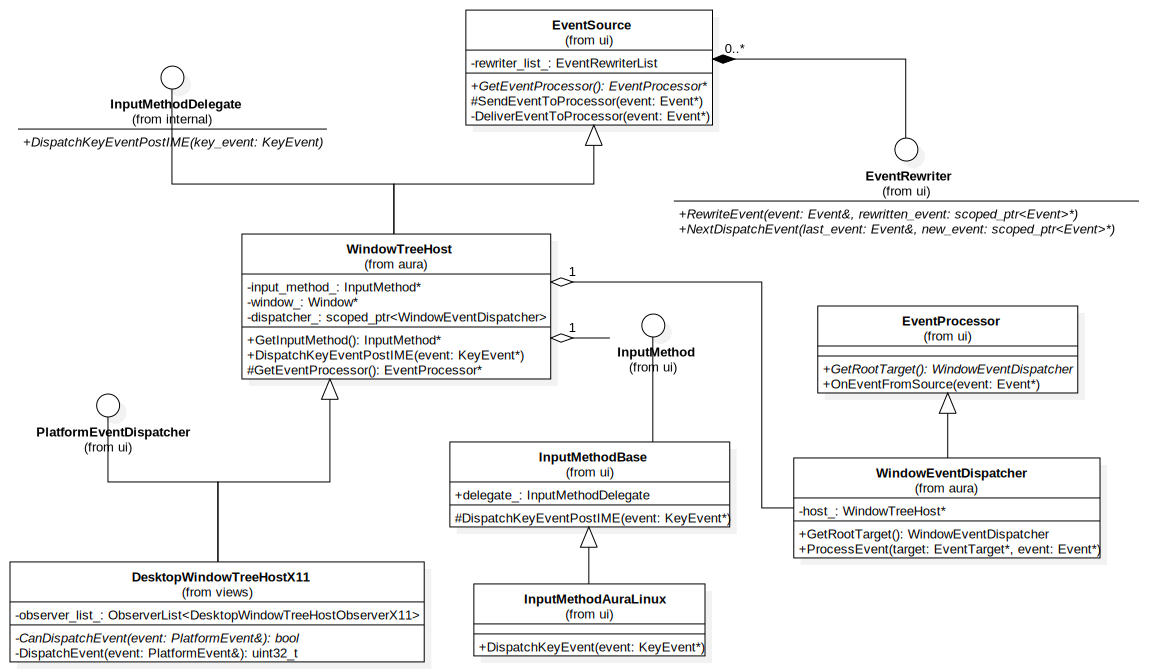
\includegraphics[width=\textwidth]{image/event_study/browser_event_dispatch_class_1.pdf} 
  \caption{chromium browser进程事件传递静态类图-1} \label{fig:linux_event_dispatch_class_1} 
\end{figure}

图~\ref{fig:linux_event_dispatch_class_1}是按键事件从PlatformEventSource到按键分发到特定window之前,
所涉及的主要类的静态类图。
\begin{itemize}
  \item DesktopWindowTreeHostX11类实现PlatformEventDispatcher接口,同时又继承了WindowTreeHost和EventSource。
  这样DesktopWindowTreeHostX11类在broeser进程中就扮演了重要的角色,可谓身兼数职。
  在事件处理流程上看它既是PlatformEventSource的dispatcher,又是UI系统的EventSource。
  \item EventSource中包含EventRewriter对象,可以在事件处理前改写事件。
  \item InputMethodBase内存在WindowTreeHost的引用。
\end{itemize}

\begin{figure}[H] 
  \centering 
  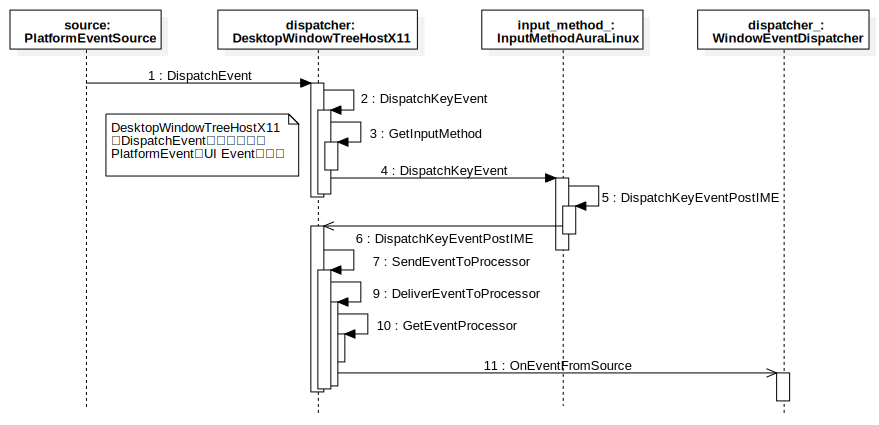
\includegraphics[width=\textwidth]{image/event_study/browser_event_dispatch_sequence_1.pdf} 
  \caption{chromium browser进程事件传递时序图-1} \label{fig:browser_event_dispatch_sequence_1} 
\end{figure}

图~\ref{fig:browser_event_dispatch_sequence_1}
是按键事件从PlatformEventSource到按键分发到特定window之前的调用时序图。

\begin{itemize}
  \item 在第1步调用中(DispatchEvent)就完成了由PlatformEvent到ui::Event的转换。
  也就屏蔽了平台层的事件,转换为chromium内部的事件类型。
  \item DesktopWindowTreeHostX11中的大部分调用都在其父类和祖父类中实现的。
  \item OnEventFromSource函数在WindowEventDispatcher的父类中实现。
\end{itemize}

\begin{spacing}{1.0}
\begin{lstlisting}[language={C++}]
    case KeyPress: {
      ui::KeyEvent keydown_event(xev);
      DispatchKeyEvent(&keydown_event);
      break;
    }
    case KeyRelease: {
      // There is no way to deactivate a window in X11 so ignore input if
      // window is supposed to be 'inactive'. See comments in
      // X11DesktopHandler::DeactivateWindow() for more details.
      if (!IsActive() && !HasCapture())
        break;

      ui::KeyEvent key_event(xev);
      DispatchKeyEvent(&key_event);
      break;
    }
\end{lstlisting}
\end{spacing}

%---------------------------------------------------------------------

\begin{figure}[H] 
  \centering 
  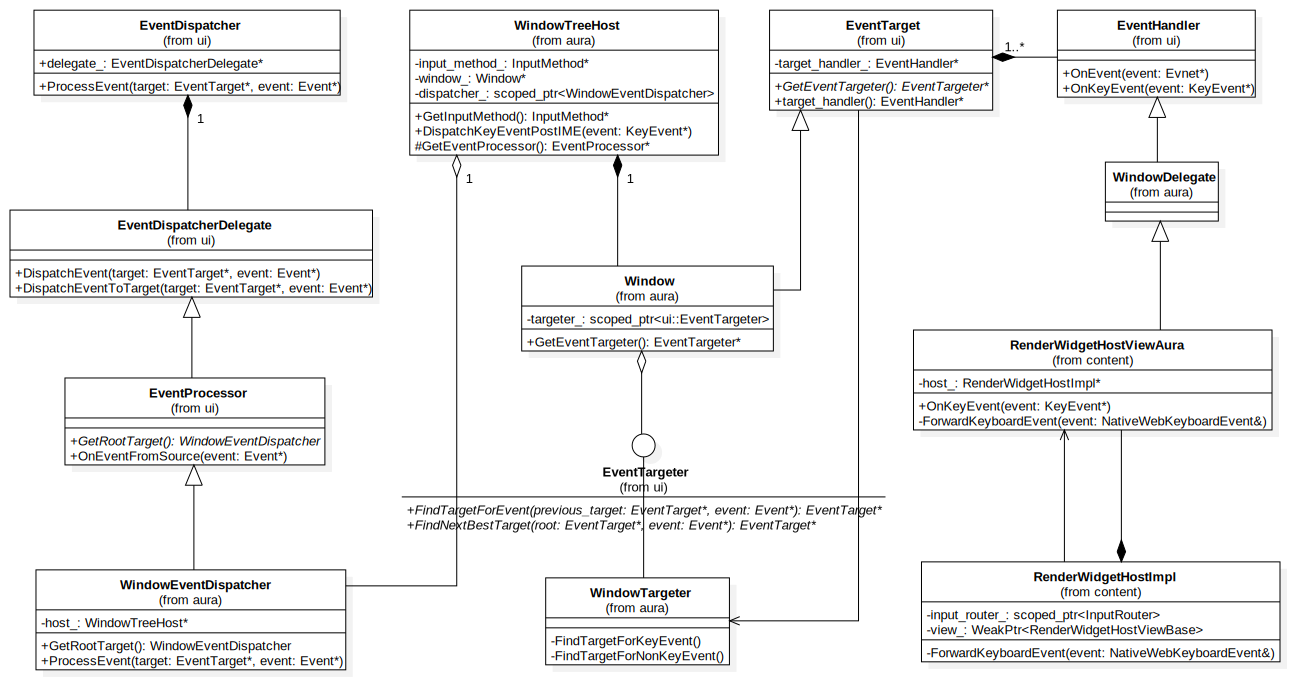
\includegraphics[width=\textwidth]{image/event_study/browser_event_dispatch_class_2.pdf} 
  \caption{chromium browser进程事件传递静态类图-2} \label{fig:linux_event_dispatch_class_2} 
\end{figure}

如图~\ref{fig:linux_event_dispatch_class_2}所示:
是按键事件由UI抽象的EventSource到与Render进程相对应的类RenderWidgetHostImpl之间所涉及的静态类图,其中:
\begin{itemize}
  \item WindowTreeHost继承了EventSource,通过实例化其子类DesktopWindowTreeHostX11来充当UI抽象的事件源。
  \item EventDispatcher和EventDispatcherDelegate是事件分发工作的主要执行者,
  EventDispatcherDelegate类实例化的是其子类WindowEventDispatcher。
  \item window继承自EventTarget可以作为事件的目标,同时又包含EventTargeter对象,用来筛选合适的window处理事件。
  \item EventTarget中实际处理事件的对象是EventHandler。EventTarget中包含3类handler,其中主处理handler仅有一个
  是target\_handler。在主handler处理前会有pre\_target\_list\_中的handler尝试处理事件,
  主handler处理后由post\_target\_list\_尝试处理。这里的处理大部分是指传递给Render进程。
  \item RenderWidgetHostViewAura类继承EventHandler,具有处理事件的能力。通过调试代码发现并不是所有的window内的\\
  target\_handler都是RenderWidgetHostViewAura。
  目前的结论是一个Render进程中的所有window只有一个target\_handler是RenderWidgetHostViewAura。
  \item RenderWidgetHostImpl与Render进程中的RenderWidget对应。
\end{itemize}

\begin{figure}[H] 
  \centering 
  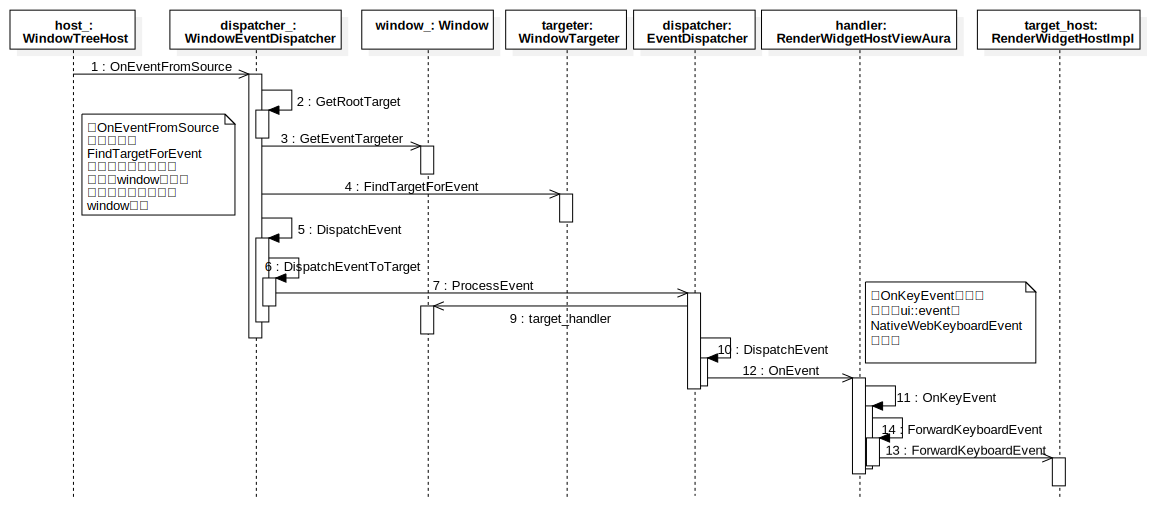
\includegraphics[width=\textwidth]{image/event_study/browser_event_dispatch_sequence_2.pdf} 
  \caption{chromium browser进程事件传递时序图-2} \label{fig:browser_event_dispatch_sequence_2} 
\end{figure}

图~\ref{fig:browser_event_dispatch_sequence_2}
是按键事件从PlatformEventSource到按键分发到特定window之前的调用时序图。

\begin{itemize}
  \item dispatcher\_对象的调用一些方法实现在其父类和祖父类中。
  其中调用GetRootTarget方法返回的对象就是root window。
  \item WindowTargeter类的FindTargetForEvent方法返回合适的window对象作为事件的target。
  由于window是树状结构,处理是会循环调用FindNextBestTarget方法。
  \item RenderWidgetHostViewAura类中的OnKeyEvent方法中完成ui::KeyEvent到NativeWebKeyboardEvent转换,
  NativeWebKeyboardEvent又是blink::WebKeyboardEvent的子类。
  所以按键事件是通过WebKeyboardEvent的形式传递给Render进程的。
\end{itemize}

\begin{spacing}{1.0}
\begin{lstlisting}[language={C++}]
if (!event_to_dispatch->handled())
target = targeter->FindTargetForEvent(root, event_to_dispatch);

EventDispatchDetails details;
while (target) {
details = DispatchEvent(target, event_to_dispatch);

...
  
target = targeter->FindNextBestTarget(target, event_to_dispatch);
}
\end{lstlisting}
\end{spacing}

%---------------------------------------------------------------------

\begin{figure}[H] 
  \centering 
  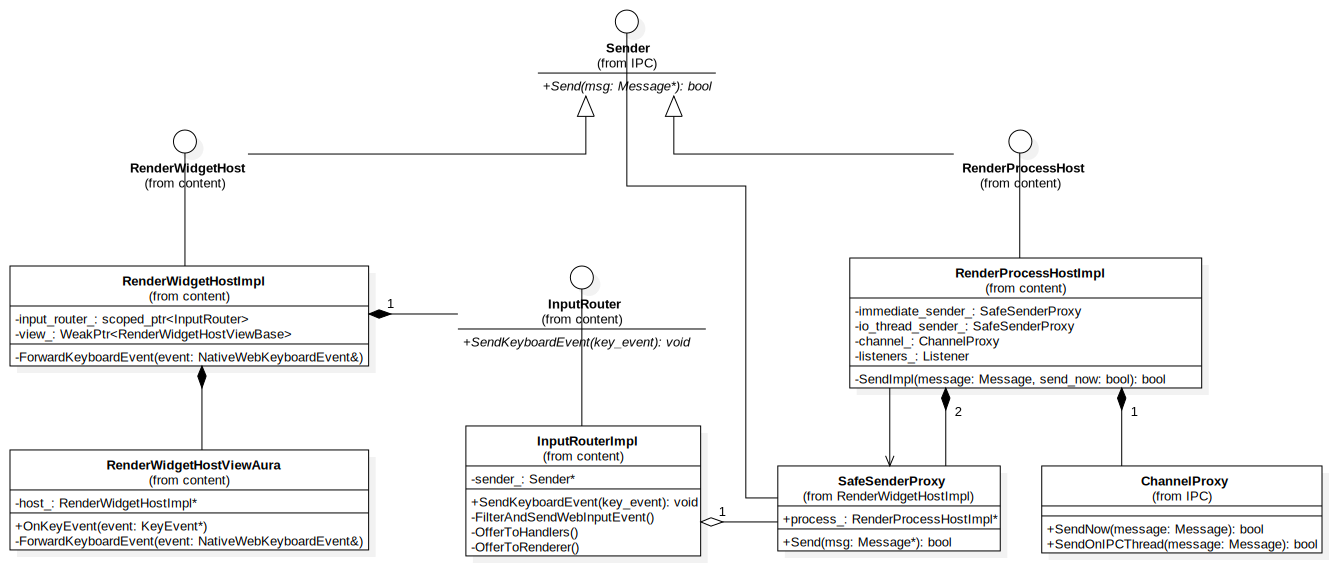
\includegraphics[width=\textwidth]{image/event_study/browser_event_dispatch_class_3.pdf} 
  \caption{chromium browser进程事件传递静态类图-3} \label{fig:browser_event_dispatch_class_3} 
\end{figure}

如图~\ref{fig:browser_event_dispatch_class_3}所示:
是browser进程发送按键消息到render进程过程中涉及的类的静态类图,其中:
\begin{itemize}
  \item RenderWidgetHostImpl、InputRouter、RenderProcessHost等类同时也继承了Listener接口,
  用于接收render进程的消息。
  \item RenderWidgetHost与Render进程中的RenderWidget对应,在chromium给出的多进程框架示意图中可以看出
  一个render进程可以存在多个RenderWidget,但只有一个RenderProcess负责与browser进程通信。
  同样,每个render进程在browser进程中都有一个RenderProcessHost。
  \item 发送消息的具体实施者是ChannelProxy类,在browser进程中实例化的ChannelProxy对象只能发送异步消息,
  后来chromium有在对象内部添加了发送同步消息的函数,但是对外的接口仍默认是异步消息。
  \item 发送消息的底层实现并没有在这里体现,留待后续研究。
\end{itemize}

\newpage
\begin{figure}[H] 
  \centering 
  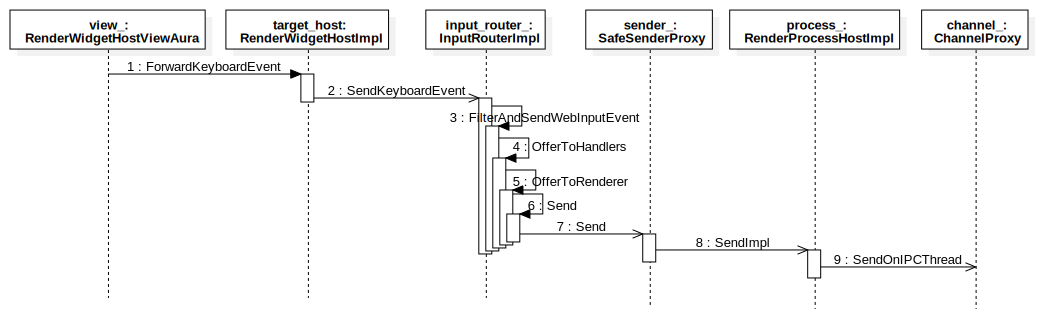
\includegraphics[width=\textwidth]{image/event_study/browser_event_dispatch_sequence_3.pdf} 
  \caption{chromium browser进程事件传递时序图-3} \label{fig:browser_event_dispatch_sequence_3} 
\end{figure}

图~\ref{fig:browser_event_dispatch_sequence_3}
是browser进程发送按键消息到render进程过程中的调用时序图,其中:

\begin{itemize}
  \item SendImpl调用SendOnIPCThread是发送异步消息,同步消息是调用SendNow。
\end{itemize}

\begin{spacing}{1.0}
\begin{lstlisting}[language={C++}]
bool RenderProcessHostImpl::SendImpl(std::unique_ptr<IPC::Message> msg,
                                     bool send_now) {
#if !defined(OS_ANDROID)
  DCHECK(!msg->is_sync());
#endif
  if (!channel_) {
#if defined(OS_ANDROID)
    if (msg->is_sync())
      return false;
#endif
    if (!is_initialized_) {
      queued_messages_.emplace(std::move(msg));
      return true;
    } else {
      return false;
    }
  }

  if (child_process_launcher_.get() && child_process_launcher_->IsStarting()) {
#if defined(OS_ANDROID)
    if (msg->is_sync())
      return false;
#endif
    queued_messages_.emplace(std::move(msg));
    return true;
  }

  if (send_now)
    return channel_->SendNow(std::move(msg));

  return channel_->SendOnIPCThread(std::move(msg));
}
\end{lstlisting}
\end{spacing}

%---------------------------------------------------------------------

\section{按键事件处理流程}
这里的按键事件处理流程指的是render进程接收到按键事件之后的处理流程。
大致过程是从brower进程获取事件;查找事件处理的页面、节点;调用节点注册的监听函数处理事件。

%---------------------------------------------------------------------

\begin{figure}[H] 
  \centering 
  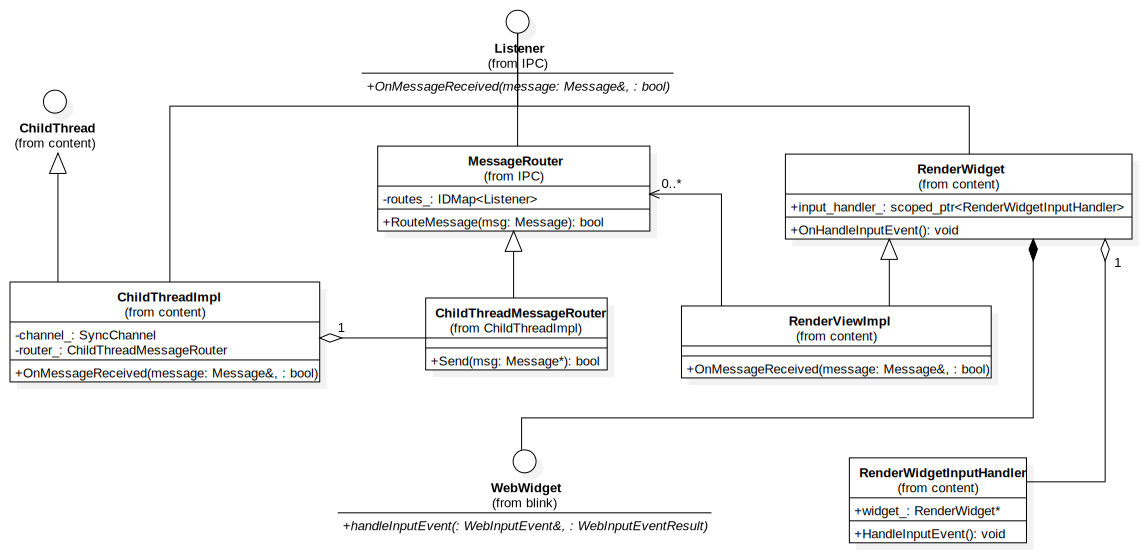
\includegraphics[width=\textwidth]{image/event_study/render_event_dispatch_class.pdf} 
  \caption{chromium render进程处理事件类图-1} \label{fig:render_event_dispatch_class} 
\end{figure}

如图~\ref{fig:render_event_dispatch_class}所示:
是browser进程的按键消息到达render进程后的,到传递给render进程中的特定WebView处理之前所涉及的类的静态类图。其中:
\begin{itemize}
  \item ChildThread、MessageRouter、RenderWidget等类同时也继承了Sender接口,用于发送消息到其他进程。
  \item 消息最先到达ChildThread的OnMessageReceived函数,在这里会处理一些消息,
  剩余消息交于ChildThreadMessageRouter处理。MessageRouter将事件传递给RenderViewImpl处理,
  RenderViewImpl也会处理一些消息,其余交于其父类RenderWidget处理,按键事件最终会传递给RenderWidget。
  \item ChildThreadImpl中的channel实例是SyncChannel对象,可以发送同步消息。
  \item 接收消息的底层实现并没有在这里体现,留待后续研究。
\end{itemize}

\newpage
\begin{figure}[H] 
  \centering 
  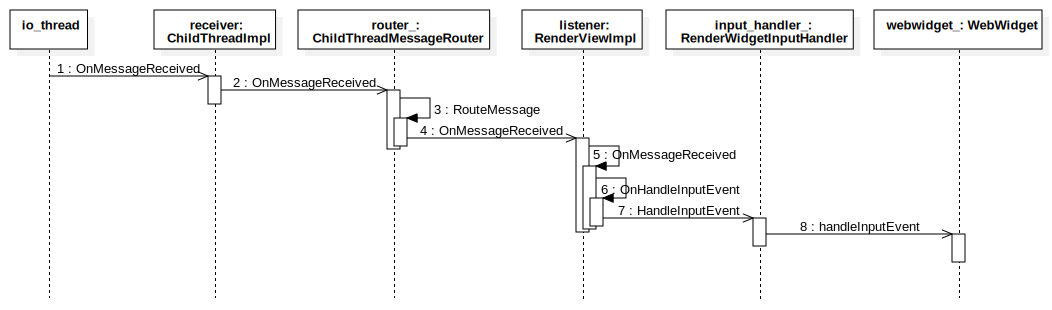
\includegraphics[width=\textwidth]{image/event_study/render_event_dispatch_sequence.pdf} 
  \caption{chromium render进程处理事件时序图-1} \label{fig:render_event_dispatch_sequence} 
\end{figure}

图~\ref{fig:render_event_dispatch_sequence}
是browser进程的按键消息到达render进程后的,到传递给render进程中的特定WebView处理之前的调用时序图,其中:

\begin{itemize}
  \item 在MessageRouter中的RouteMessage中选择哪个RenderView处理事件。
  \item RenderWidgetInputHandler调用RenderWidget的接口获取RenderWidget的webwidget\_处理事件。
\end{itemize}

\begin{spacing}{1.0}
\begin{lstlisting}[language={C++}]
bool MessageRouter::RouteMessage(const IPC::Message& msg) {
  IPC::Listener* listener = routes_.Lookup(msg.routing_id());
  if (!listener)
    return false;

  return listener->OnMessageReceived(msg);
}

void RenderWidgetInputHandler::HandleInputEvent(
    const WebInputEvent& input_event,
    const ui::LatencyInfo& latency_info,
    InputEventDispatchType dispatch_type) {
  ...
  
  WebInputEventResult processed = prevent_default
                                      ? WebInputEventResult::HandledSuppressed
                                      : WebInputEventResult::NotHandled;
  if (input_event.type != WebInputEvent::Char || !suppress_next_char_events_) {
    suppress_next_char_events_ = false;
    if (processed == WebInputEventResult::NotHandled && widget_->webwidget())
      processed = widget_->webwidget()->handleInputEvent(input_event);
  }
  ...  
}
\end{lstlisting}
\end{spacing}

%---------------------------------------------------------------------

\begin{figure}[H] 
  \centering 
  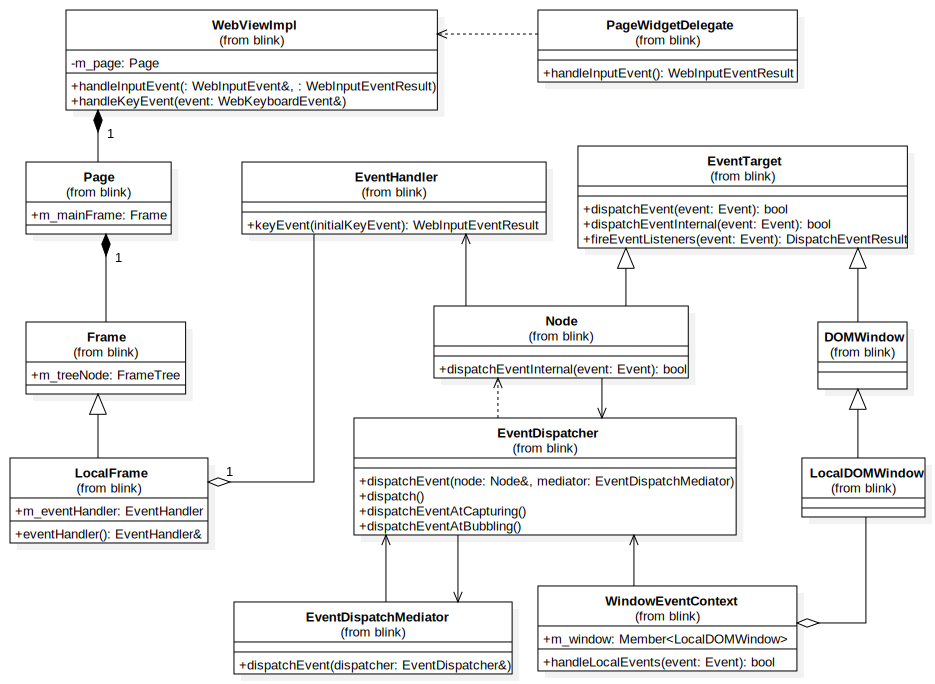
\includegraphics[width=\textwidth]{image/event_study/render_event_handle_class.pdf} 
  \caption{chromium render进程处理事件类图-2} \label{fig:render_event_handle_class} 
\end{figure}

如图~\ref{fig:render_event_handle_class}所示:
是render进程的渲染引擎blink处理按键事件过程中涉及的类的静态类图。其中:
\begin{itemize}
  \item WebViewImpl实现WebWidget接口和WebView接口功能,是RenderWidget的成员变量。
  传递给它的事件将传递给其成员变量m\_page。
  \item 在一个Page中可能包含多个Frame,Page将选择合适的Frame处理传入的事件。
  事件将交于Frame中的m\_eventHandler变量处理。
  \item 在EventHandler中,将遍历DOM树,查找合适的Node处理事件。
  最终通过Node的父类EventTarget调用所以注册的监听函数。
  \item 此过程使用的类都属于blink命名空间,是原来的WebKit内核代码。
\end{itemize}

\newpage
\begin{figure}[H] 
  \centering 
  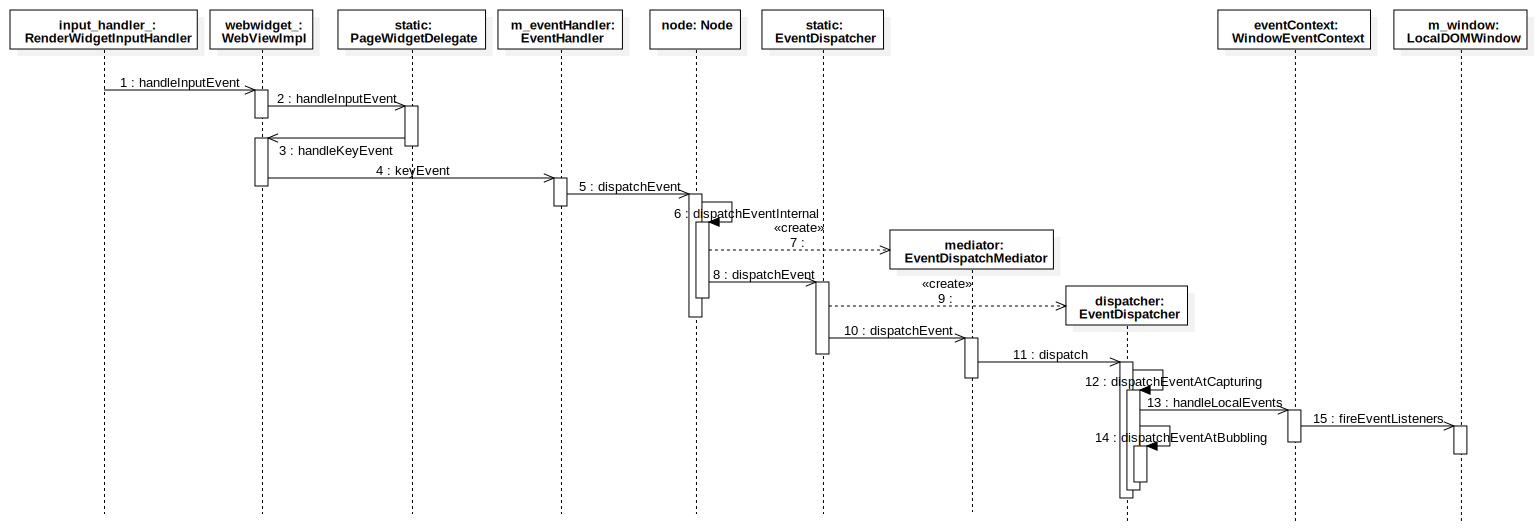
\includegraphics[width=\textwidth]{image/event_study/render_event_handle_sequence.pdf} 
  \caption{chromium render进程处理事件时序图-2} \label{fig:render_event_handle_sequence} 
\end{figure}

图~\ref{fig:render_event_handle_sequence}
是render进程的渲染引擎blink处理按键事件流程调用时序图,其中:
\begin{itemize}
  \item 第3步handleKeyEvent在调用keyEvent方法处理后,若无处理将调用keyEventDefault进行事件的默认处理。
  \item 第4步keyEvent方法中将调用eventTargetNodeForDocument函数,用来查找合适的Node来处理事件。
  \item 第11步EventDispatcher的dispatch方法中首先调用dispatchEventAtCapturing进行事件捕获,
  然后调用dispatchEventAtBubbling进行事件冒泡,这些过程中都会检查事件是否要继续处理。
\end{itemize}

\begin{spacing}{1.0}
\begin{lstlisting}[language={C++}]
DispatchEventResult EventDispatcher::dispatch()
{
    ...
    
    EventDispatchHandlingState* preDispatchEventHandlerResult = nullptr;
    if (dispatchEventPreProcess(preDispatchEventHandlerResult) == ContinueDispatching) {
        if (dispatchEventAtCapturing() == ContinueDispatching) {
            if (dispatchEventAtTarget() == ContinueDispatching)
                dispatchEventAtBubbling();
        }
    }
    
    ...
    return EventTarget::dispatchEventResult(*m_event);
}
\end{lstlisting}
\end{spacing}

%---------------------------------------------------------------------

\ifx\withtbrowser\undefined
\else
\section{引言}
众所周知,chromium是多线程框架的,整个chromium浏览器包括四类进程:browser主进程、render渲染进程、GPU进程和插件进程。
本文所要讲述的chromium事件处理流程主要牵涉到其中的两种进程:browser进程和render进程。

事件处理的大体流程是由browser进程接收并传递给render进程处理。
然而我们知道render会不止一个,那么browser进程如何获取事件?
又如何传递给特定的render进程?render进程如何处理事件消息?我们下面就通过分析代码来一一探明。

chromium系统有多个平台的实现,而每个平台都有自己不同的事件管理方式,chromium也会有一些平台相关的代码。
本文目前主要是研究Linux平台相关的实现,其他平台后续再做研究。
chromium中的事件也有许多类型,如按键事件、鼠标事件、滚轮事件等等。
本文也只是以按键事件为例研究,在以下内容中,如无特殊说明,事件均指的是按键事件。

\section{按键事件获取流程}
\begin{figure}[H] 
  \centering 
  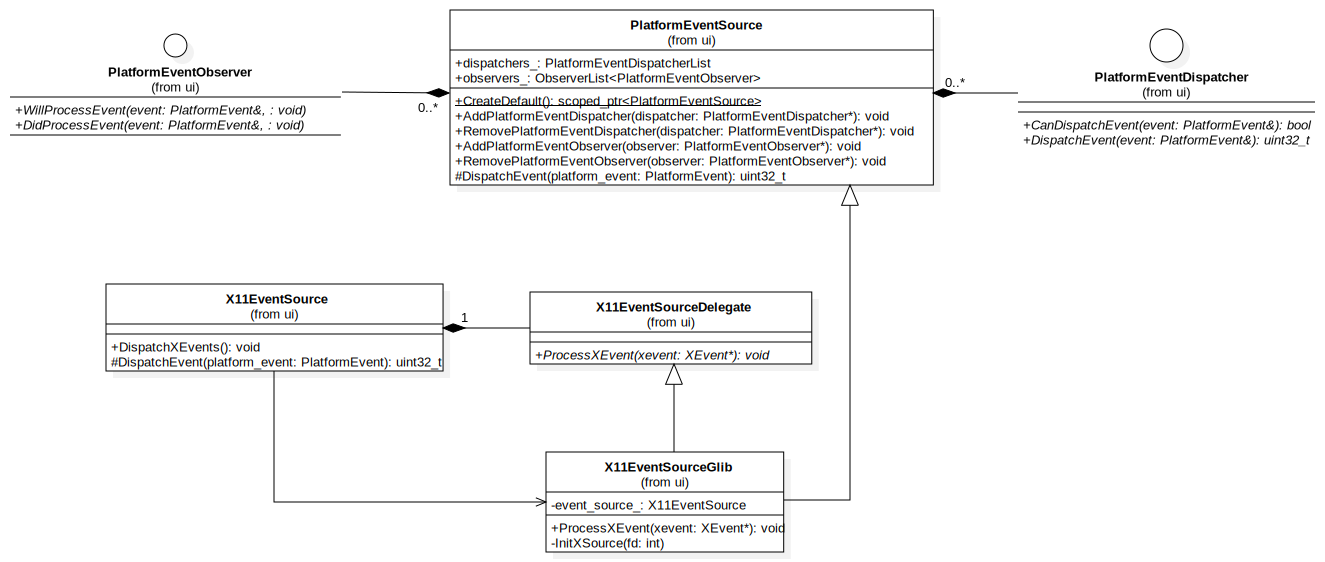
\includegraphics[width=\textwidth]{image/event_study/linux_event_source_class.pdf} 
  \caption{chromium linux平台事件源静态类图} \label{fig:linux_event_source_class} 
\end{figure}

如第图~\ref{fig:linux_event_source_class}所示:
chromium对事件源抽象了一个PlatformEventSource类表示,不同的平台继承该类实现自己平台的子类。
不过,目前发现仅有Linux平台实现了其子类X11EventSource与X11EventSourceGlib。
Windows和Android都未采用该方法。

\begin{figure}[H] 
  \centering 
  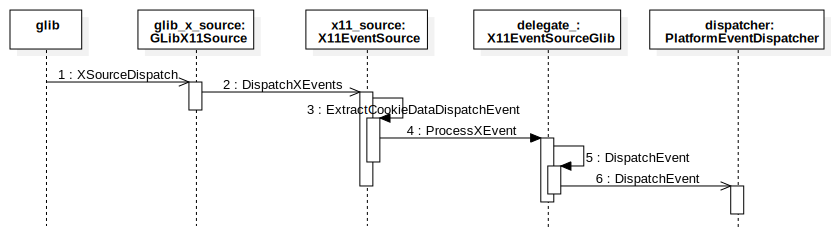
\includegraphics[width=\textwidth]{image/event_study/linux_get_event_from_source.pdf} 
  \caption{chromium linux平台事件获取时序图} \label{fig:linux_get_event_from_source} 
\end{figure}

browser进程获取按键事件的调用时序图如图~\ref{fig:linux_get_event_from_source}所示:
\begin{itemize}
  \item 在browser进程启动时,会创建一个线程循环调用g\_main\_context\_iteration方法。其作用是驱动glib检查事件,如果有事件发生,则glib会调用初始化时注册的XSourceDispatch回调来将事件传递给PlatformEventSource的子类。
  \item 第5步调用时是调用的父类PlatformEventSource方法,将事件传递给PlatformEventDispatcher。
\end{itemize}

\begin{spacing}{1.0}
\begin{lstlisting}[language={C++}]
  for (;;) {
    // Don't block if we think we have more work to do.
    bool block = !more_work_is_plausible;

    more_work_is_plausible = g_main_context_iteration(context_, block);
    if (state_->should_quit)
      break;

    more_work_is_plausible |= state_->delegate->DoWork();
    if (state_->should_quit)
      break;

    more_work_is_plausible |=
        state_->delegate->DoDelayedWork(&delayed_work_time_);
    if (state_->should_quit)
      break;

    if (more_work_is_plausible)
      continue;

    more_work_is_plausible = state_->delegate->DoIdleWork();
    if (state_->should_quit)
      break;
  }
\end{lstlisting}
\end{spacing}

\section{按键事件传递流程}
这里的按键传递流程是指browser进程从事件源处取得事件之后将其传递给特定的render进程的过程。
这里研究的是使用chromium的aura窗口系统的流程,平台是Linux平台,
然而据初步研究Windows和Android也是使用同样的流程,只是传入事件的位置不同罢了。

%---------------------------------------------------------------------

\begin{figure}[H] 
  \centering 
  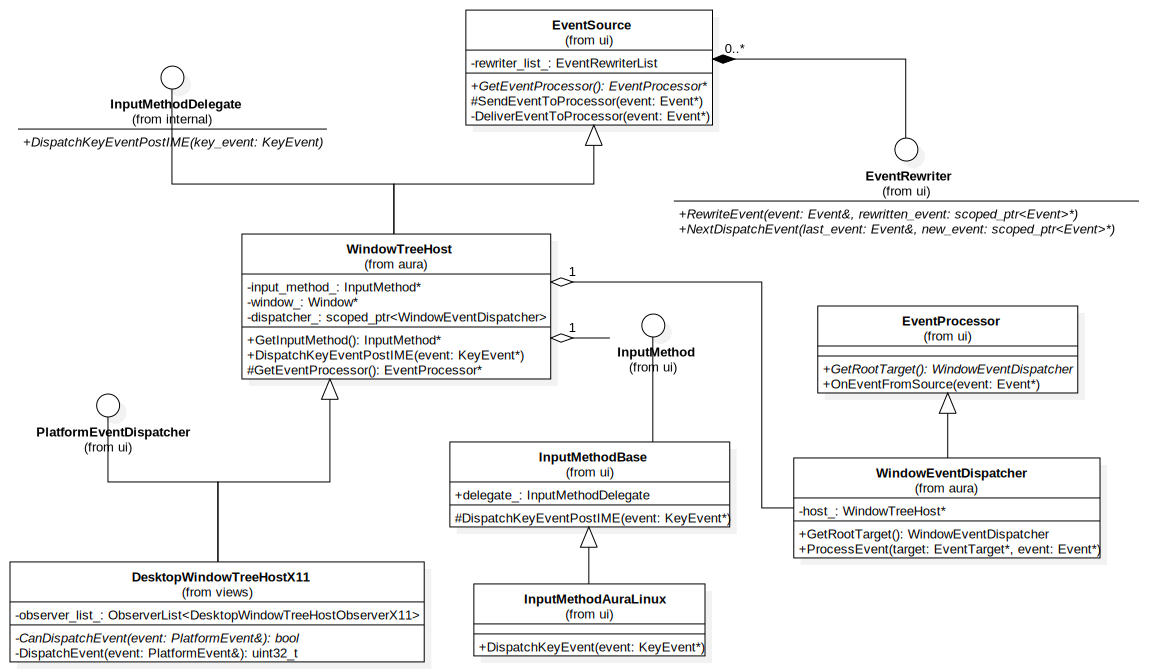
\includegraphics[width=\textwidth]{image/event_study/browser_event_dispatch_class_1.pdf} 
  \caption{chromium browser进程事件传递静态类图-1} \label{fig:linux_event_dispatch_class_1} 
\end{figure}

图~\ref{fig:linux_event_dispatch_class_1}是按键事件从PlatformEventSource到按键分发到特定window之前,
所涉及的主要类的静态类图。
\begin{itemize}
  \item DesktopWindowTreeHostX11类实现PlatformEventDispatcher接口,同时又继承了WindowTreeHost和EventSource。
  这样DesktopWindowTreeHostX11类在broeser进程中就扮演了重要的角色,可谓身兼数职。
  在事件处理流程上看它既是PlatformEventSource的dispatcher,又是UI系统的EventSource。
  \item EventSource中包含EventRewriter对象,可以在事件处理前改写事件。
  \item InputMethodBase内存在WindowTreeHost的引用。
\end{itemize}

\begin{figure}[H] 
  \centering 
  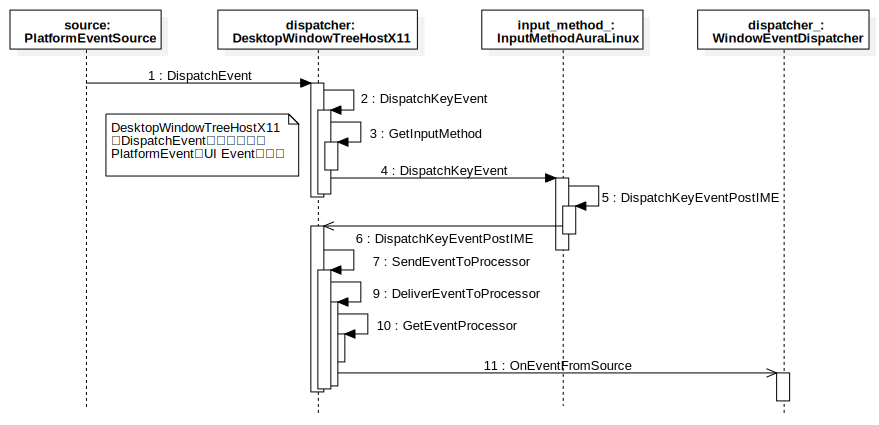
\includegraphics[width=\textwidth]{image/event_study/browser_event_dispatch_sequence_1.pdf} 
  \caption{chromium browser进程事件传递时序图-1} \label{fig:browser_event_dispatch_sequence_1} 
\end{figure}

图~\ref{fig:browser_event_dispatch_sequence_1}
是按键事件从PlatformEventSource到按键分发到特定window之前的调用时序图。

\begin{itemize}
  \item 在第1步调用中(DispatchEvent)就完成了由PlatformEvent到ui::Event的转换。
  也就屏蔽了平台层的事件,转换为chromium内部的事件类型。
  \item DesktopWindowTreeHostX11中的大部分调用都在其父类和祖父类中实现的。
  \item OnEventFromSource函数在WindowEventDispatcher的父类中实现。
\end{itemize}

\begin{spacing}{1.0}
\begin{lstlisting}[language={C++}]
    case KeyPress: {
      ui::KeyEvent keydown_event(xev);
      DispatchKeyEvent(&keydown_event);
      break;
    }
    case KeyRelease: {
      // There is no way to deactivate a window in X11 so ignore input if
      // window is supposed to be 'inactive'. See comments in
      // X11DesktopHandler::DeactivateWindow() for more details.
      if (!IsActive() && !HasCapture())
        break;

      ui::KeyEvent key_event(xev);
      DispatchKeyEvent(&key_event);
      break;
    }
\end{lstlisting}
\end{spacing}

%---------------------------------------------------------------------

\begin{figure}[H] 
  \centering 
  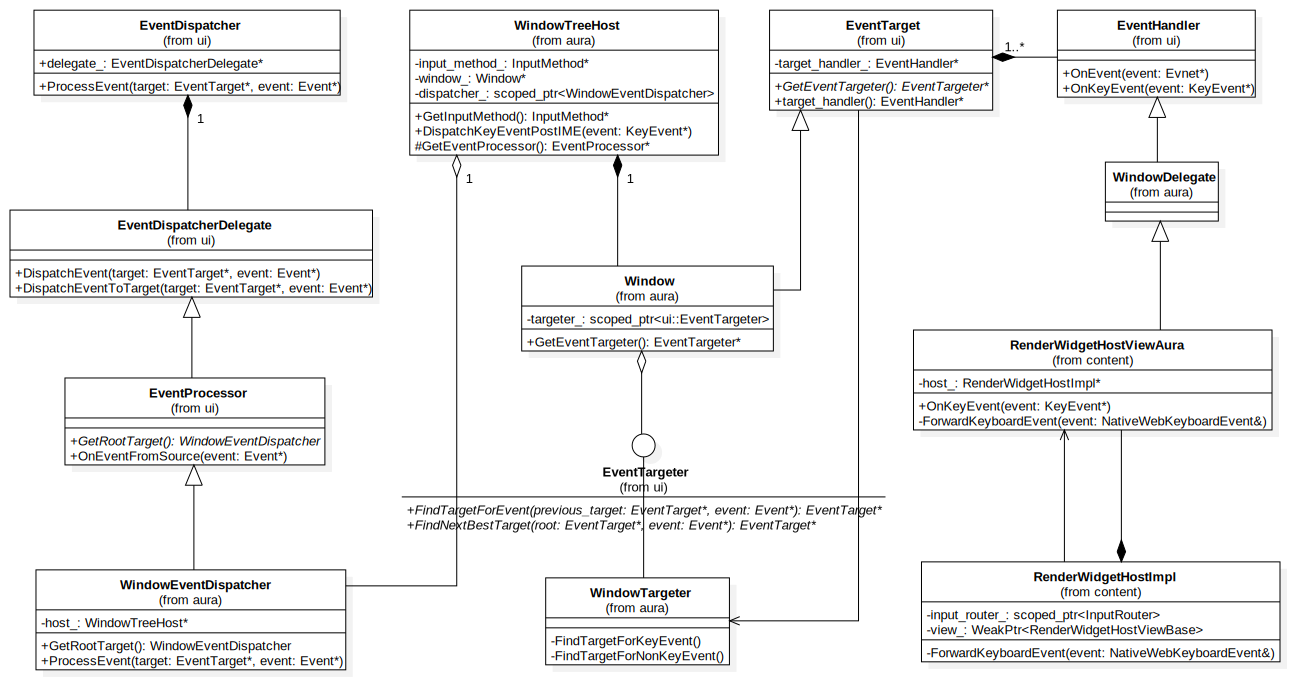
\includegraphics[width=\textwidth]{image/event_study/browser_event_dispatch_class_2.pdf} 
  \caption{chromium browser进程事件传递静态类图-2} \label{fig:linux_event_dispatch_class_2} 
\end{figure}

如图~\ref{fig:linux_event_dispatch_class_2}所示:
是按键事件由UI抽象的EventSource到与Render进程相对应的类RenderWidgetHostImpl之间所涉及的静态类图,其中:
\begin{itemize}
  \item WindowTreeHost继承了EventSource,通过实例化其子类DesktopWindowTreeHostX11来充当UI抽象的事件源。
  \item EventDispatcher和EventDispatcherDelegate是事件分发工作的主要执行者,
  EventDispatcherDelegate类实例化的是其子类WindowEventDispatcher。
  \item window继承自EventTarget可以作为事件的目标,同时又包含EventTargeter对象,用来筛选合适的window处理事件。
  \item EventTarget中实际处理事件的对象是EventHandler。EventTarget中包含3类handler,其中主处理handler仅有一个
  是target\_handler。在主handler处理前会有pre\_target\_list\_中的handler尝试处理事件,
  主handler处理后由post\_target\_list\_尝试处理。这里的处理大部分是指传递给Render进程。
  \item RenderWidgetHostViewAura类继承EventHandler,具有处理事件的能力。通过调试代码发现并不是所有的window内的\\
  target\_handler都是RenderWidgetHostViewAura。
  目前的结论是一个Render进程中的所有window只有一个target\_handler是RenderWidgetHostViewAura。
  \item RenderWidgetHostImpl与Render进程中的RenderWidget对应。
\end{itemize}

\begin{figure}[H] 
  \centering 
  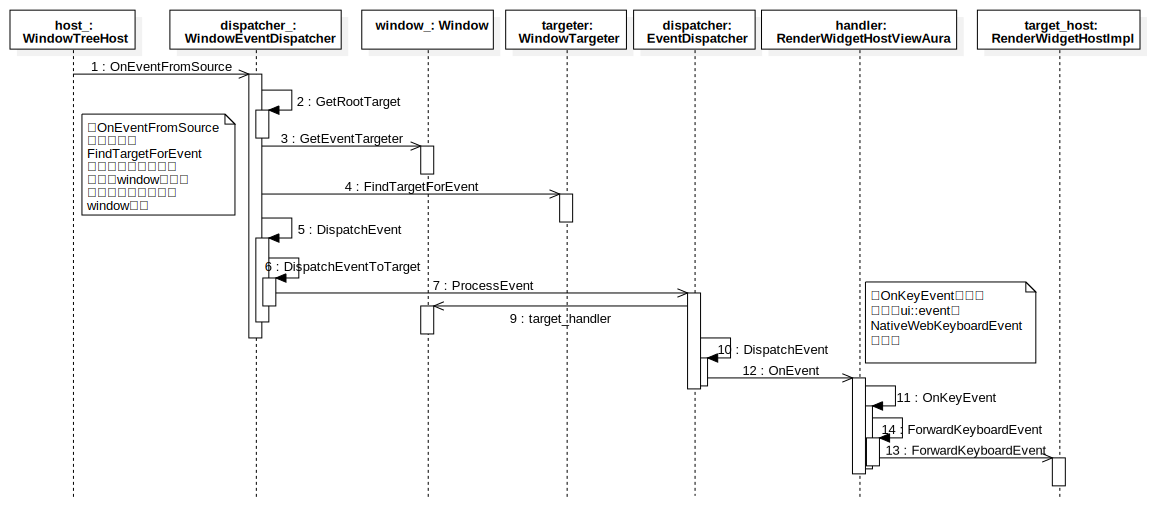
\includegraphics[width=\textwidth]{image/event_study/browser_event_dispatch_sequence_2.pdf} 
  \caption{chromium browser进程事件传递时序图-2} \label{fig:browser_event_dispatch_sequence_2} 
\end{figure}

图~\ref{fig:browser_event_dispatch_sequence_2}
是按键事件从PlatformEventSource到按键分发到特定window之前的调用时序图。

\begin{itemize}
  \item dispatcher\_对象的调用一些方法实现在其父类和祖父类中。
  其中调用GetRootTarget方法返回的对象就是root window。
  \item WindowTargeter类的FindTargetForEvent方法返回合适的window对象作为事件的target。
  由于window是树状结构,处理是会循环调用FindNextBestTarget方法。
  \item RenderWidgetHostViewAura类中的OnKeyEvent方法中完成ui::KeyEvent到NativeWebKeyboardEvent转换,
  NativeWebKeyboardEvent又是blink::WebKeyboardEvent的子类。
  所以按键事件是通过WebKeyboardEvent的形式传递给Render进程的。
\end{itemize}

\begin{spacing}{1.0}
\begin{lstlisting}[language={C++}]
if (!event_to_dispatch->handled())
target = targeter->FindTargetForEvent(root, event_to_dispatch);

EventDispatchDetails details;
while (target) {
details = DispatchEvent(target, event_to_dispatch);

...
  
target = targeter->FindNextBestTarget(target, event_to_dispatch);
}
\end{lstlisting}
\end{spacing}

%---------------------------------------------------------------------

\begin{figure}[H] 
  \centering 
  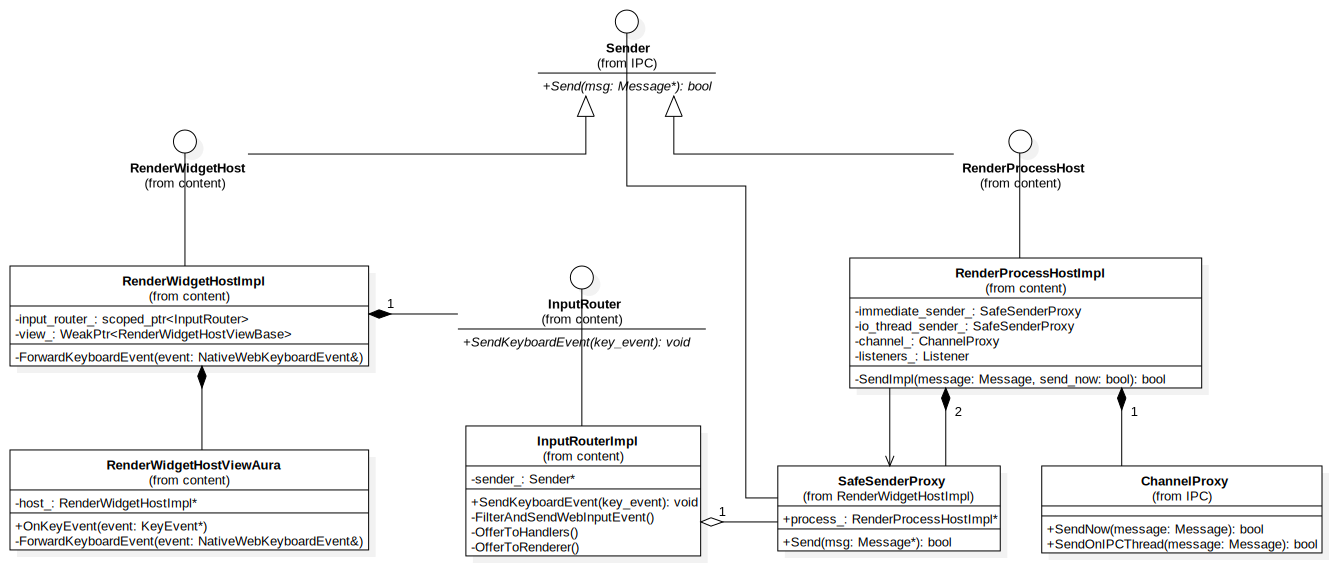
\includegraphics[width=\textwidth]{image/event_study/browser_event_dispatch_class_3.pdf} 
  \caption{chromium browser进程事件传递静态类图-3} \label{fig:browser_event_dispatch_class_3} 
\end{figure}

如图~\ref{fig:browser_event_dispatch_class_3}所示:
是browser进程发送按键消息到render进程过程中涉及的类的静态类图,其中:
\begin{itemize}
  \item RenderWidgetHostImpl、InputRouter、RenderProcessHost等类同时也继承了Listener接口,
  用于接收render进程的消息。
  \item RenderWidgetHost与Render进程中的RenderWidget对应,在chromium给出的多进程框架示意图中可以看出
  一个render进程可以存在多个RenderWidget,但只有一个RenderProcess负责与browser进程通信。
  同样,每个render进程在browser进程中都有一个RenderProcessHost。
  \item 发送消息的具体实施者是ChannelProxy类,在browser进程中实例化的ChannelProxy对象只能发送异步消息,
  后来chromium有在对象内部添加了发送同步消息的函数,但是对外的接口仍默认是异步消息。
  \item 发送消息的底层实现并没有在这里体现,留待后续研究。
\end{itemize}

\newpage
\begin{figure}[H] 
  \centering 
  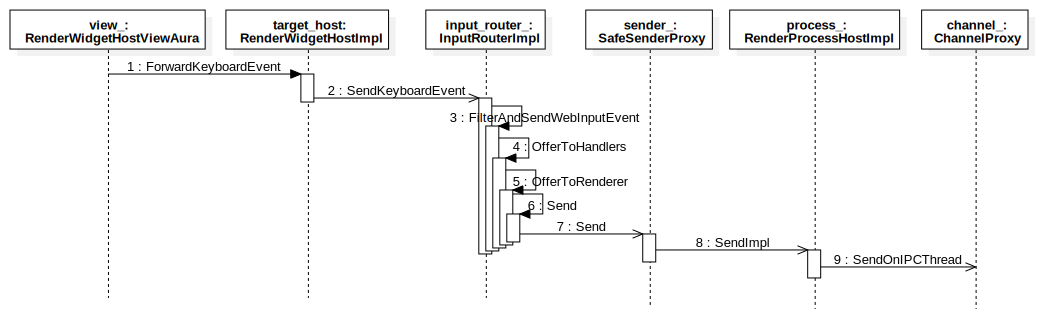
\includegraphics[width=\textwidth]{image/event_study/browser_event_dispatch_sequence_3.pdf} 
  \caption{chromium browser进程事件传递时序图-3} \label{fig:browser_event_dispatch_sequence_3} 
\end{figure}

图~\ref{fig:browser_event_dispatch_sequence_3}
是browser进程发送按键消息到render进程过程中的调用时序图,其中:

\begin{itemize}
  \item SendImpl调用SendOnIPCThread是发送异步消息,同步消息是调用SendNow。
\end{itemize}

\begin{spacing}{1.0}
\begin{lstlisting}[language={C++}]
bool RenderProcessHostImpl::SendImpl(std::unique_ptr<IPC::Message> msg,
                                     bool send_now) {
#if !defined(OS_ANDROID)
  DCHECK(!msg->is_sync());
#endif
  if (!channel_) {
#if defined(OS_ANDROID)
    if (msg->is_sync())
      return false;
#endif
    if (!is_initialized_) {
      queued_messages_.emplace(std::move(msg));
      return true;
    } else {
      return false;
    }
  }

  if (child_process_launcher_.get() && child_process_launcher_->IsStarting()) {
#if defined(OS_ANDROID)
    if (msg->is_sync())
      return false;
#endif
    queued_messages_.emplace(std::move(msg));
    return true;
  }

  if (send_now)
    return channel_->SendNow(std::move(msg));

  return channel_->SendOnIPCThread(std::move(msg));
}
\end{lstlisting}
\end{spacing}

%---------------------------------------------------------------------

\section{按键事件处理流程}
这里的按键事件处理流程指的是render进程接收到按键事件之后的处理流程。
大致过程是从brower进程获取事件;查找事件处理的页面、节点;调用节点注册的监听函数处理事件。

%---------------------------------------------------------------------

\begin{figure}[H] 
  \centering 
  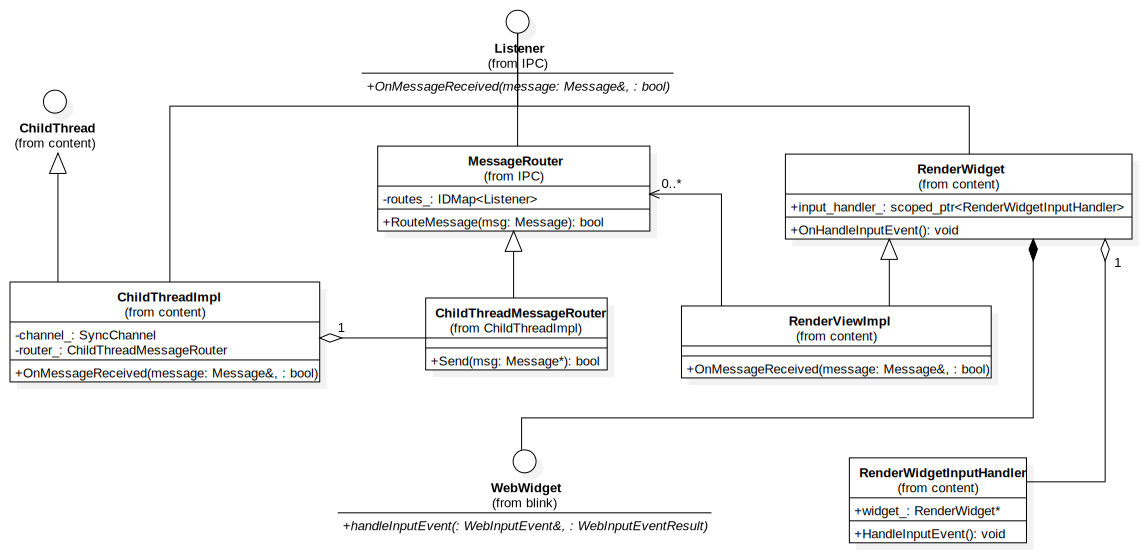
\includegraphics[width=\textwidth]{image/event_study/render_event_dispatch_class.pdf} 
  \caption{chromium render进程处理事件类图-1} \label{fig:render_event_dispatch_class} 
\end{figure}

如图~\ref{fig:render_event_dispatch_class}所示:
是browser进程的按键消息到达render进程后的,到传递给render进程中的特定WebView处理之前所涉及的类的静态类图。其中:
\begin{itemize}
  \item ChildThread、MessageRouter、RenderWidget等类同时也继承了Sender接口,用于发送消息到其他进程。
  \item 消息最先到达ChildThread的OnMessageReceived函数,在这里会处理一些消息,
  剩余消息交于ChildThreadMessageRouter处理。MessageRouter将事件传递给RenderViewImpl处理,
  RenderViewImpl也会处理一些消息,其余交于其父类RenderWidget处理,按键事件最终会传递给RenderWidget。
  \item ChildThreadImpl中的channel实例是SyncChannel对象,可以发送同步消息。
  \item 接收消息的底层实现并没有在这里体现,留待后续研究。
\end{itemize}

\newpage
\begin{figure}[H] 
  \centering 
  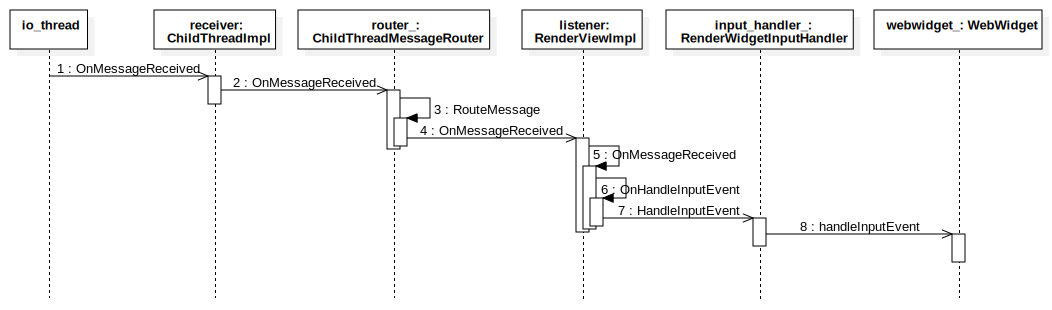
\includegraphics[width=\textwidth]{image/event_study/render_event_dispatch_sequence.pdf} 
  \caption{chromium render进程处理事件时序图-1} \label{fig:render_event_dispatch_sequence} 
\end{figure}

图~\ref{fig:render_event_dispatch_sequence}
是browser进程的按键消息到达render进程后的,到传递给render进程中的特定WebView处理之前的调用时序图,其中:

\begin{itemize}
  \item 在MessageRouter中的RouteMessage中选择哪个RenderView处理事件。
  \item RenderWidgetInputHandler调用RenderWidget的接口获取RenderWidget的webwidget\_处理事件。
\end{itemize}

\begin{spacing}{1.0}
\begin{lstlisting}[language={C++}]
bool MessageRouter::RouteMessage(const IPC::Message& msg) {
  IPC::Listener* listener = routes_.Lookup(msg.routing_id());
  if (!listener)
    return false;

  return listener->OnMessageReceived(msg);
}

void RenderWidgetInputHandler::HandleInputEvent(
    const WebInputEvent& input_event,
    const ui::LatencyInfo& latency_info,
    InputEventDispatchType dispatch_type) {
  ...
  
  WebInputEventResult processed = prevent_default
                                      ? WebInputEventResult::HandledSuppressed
                                      : WebInputEventResult::NotHandled;
  if (input_event.type != WebInputEvent::Char || !suppress_next_char_events_) {
    suppress_next_char_events_ = false;
    if (processed == WebInputEventResult::NotHandled && widget_->webwidget())
      processed = widget_->webwidget()->handleInputEvent(input_event);
  }
  ...  
}
\end{lstlisting}
\end{spacing}

%---------------------------------------------------------------------

\begin{figure}[H] 
  \centering 
  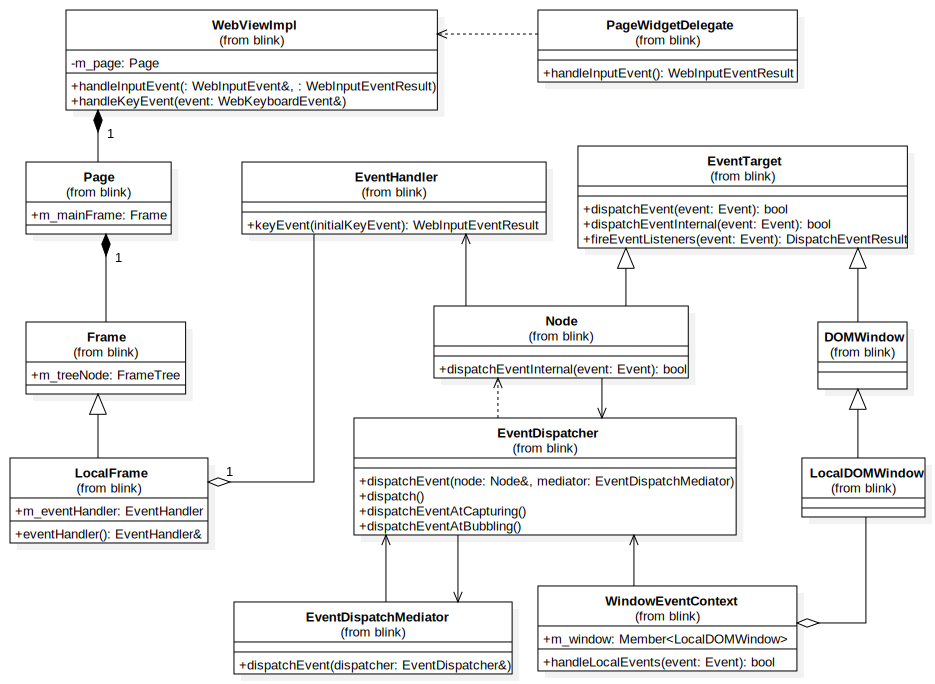
\includegraphics[width=\textwidth]{image/event_study/render_event_handle_class.pdf} 
  \caption{chromium render进程处理事件类图-2} \label{fig:render_event_handle_class} 
\end{figure}

如图~\ref{fig:render_event_handle_class}所示:
是render进程的渲染引擎blink处理按键事件过程中涉及的类的静态类图。其中:
\begin{itemize}
  \item WebViewImpl实现WebWidget接口和WebView接口功能,是RenderWidget的成员变量。
  传递给它的事件将传递给其成员变量m\_page。
  \item 在一个Page中可能包含多个Frame,Page将选择合适的Frame处理传入的事件。
  事件将交于Frame中的m\_eventHandler变量处理。
  \item 在EventHandler中,将遍历DOM树,查找合适的Node处理事件。
  最终通过Node的父类EventTarget调用所以注册的监听函数。
  \item 此过程使用的类都属于blink命名空间,是原来的WebKit内核代码。
\end{itemize}

\newpage
\begin{figure}[H] 
  \centering 
  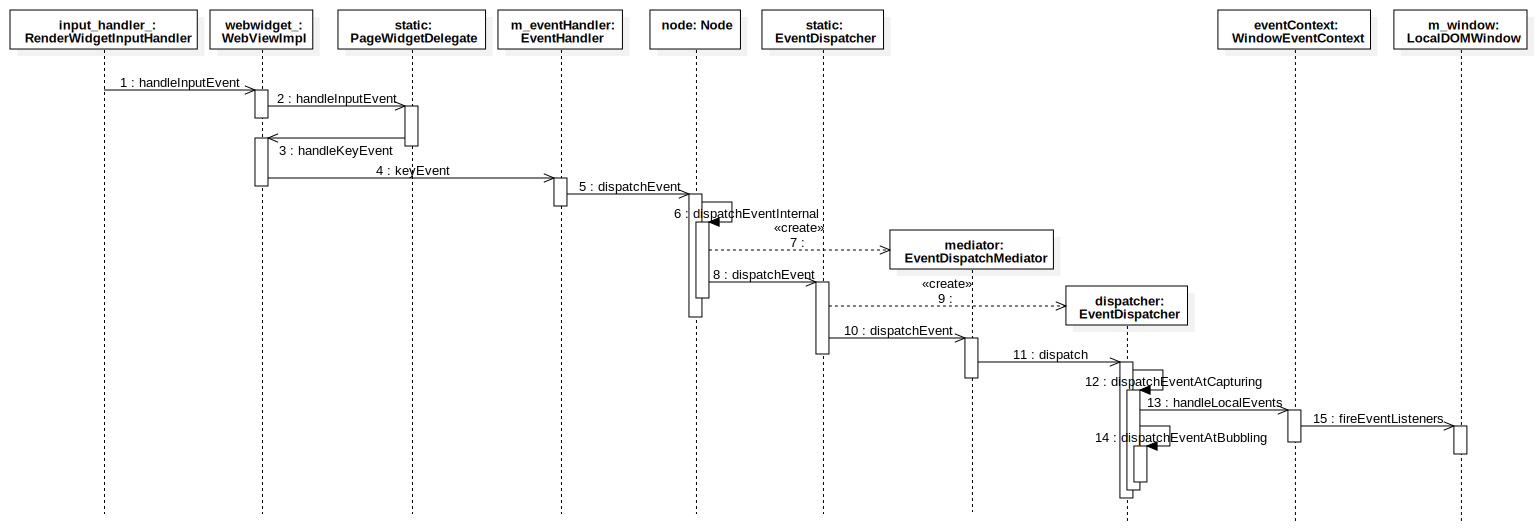
\includegraphics[width=\textwidth]{image/event_study/render_event_handle_sequence.pdf} 
  \caption{chromium render进程处理事件时序图-2} \label{fig:render_event_handle_sequence} 
\end{figure}

图~\ref{fig:render_event_handle_sequence}
是render进程的渲染引擎blink处理按键事件流程调用时序图,其中:
\begin{itemize}
  \item 第3步handleKeyEvent在调用keyEvent方法处理后,若无处理将调用keyEventDefault进行事件的默认处理。
  \item 第4步keyEvent方法中将调用eventTargetNodeForDocument函数,用来查找合适的Node来处理事件。
  \item 第11步EventDispatcher的dispatch方法中首先调用dispatchEventAtCapturing进行事件捕获,
  然后调用dispatchEventAtBubbling进行事件冒泡,这些过程中都会检查事件是否要继续处理。
\end{itemize}

\begin{spacing}{1.0}
\begin{lstlisting}[language={C++}]
DispatchEventResult EventDispatcher::dispatch()
{
    ...
    
    EventDispatchHandlingState* preDispatchEventHandlerResult = nullptr;
    if (dispatchEventPreProcess(preDispatchEventHandlerResult) == ContinueDispatching) {
        if (dispatchEventAtCapturing() == ContinueDispatching) {
            if (dispatchEventAtTarget() == ContinueDispatching)
                dispatchEventAtBubbling();
        }
    }
    
    ...
    return EventTarget::dispatchEventResult(*m_event);
}
\end{lstlisting}
\end{spacing}

%---------------------------------------------------------------------

\ifx\withtbrowser\undefined
\else
\input{contents/tbrowser/event_study.tex}
\fi

\fi

\fi

\fi
